\documentclass[11pt]{article}
\usepackage[margin=1in]{geometry}
\usepackage{amsmath,amssymb,array,booktabs,longtable,graphicx}
\usepackage[hidelinks]{hyperref}
\usepackage[T1]{fontenc}
\usepackage{lmodern}
\newcommand{\doctype}{Technical report}
\newcommand{\docversion}{v0.11.000}
\newcommand{\docdate}{31 October 2026}
\newcommand{\versiondoi}{10.5281/zenodo.NNNNNNNN}
\newcommand{\conceptdoi}{10.5281/zenodo.NNNNNNNN}
\newcommand{\docrepo}{github.com/fsantibanezleal/CAOS\_PhaseFlow}
\newcommand{\headerblock}{\begin{center}\fbox{\parbox{0.94\textwidth}{\small\raggedright
\textbf{\doctype}\quad$\cdot$\quad\docversion, \docdate\quad$\cdot$\quad Licence CC BY 4.0\\
CAOS Research, PhaseFlow open-pit production scheduling\\
Version DOI \href{https://doi.org/\versiondoi}{\texttt{\versiondoi}}\\[2pt]
Concept DOI (always latest) \href{https://doi.org/\conceptdoi}{\texttt{\conceptdoi}}\\[2pt]
Not peer reviewed. Source code, data and computational records:\\
\href{https://\docrepo}{\texttt{\docrepo}}
}}\end{center}\vspace{4pt}}
\title{PhaseFlow: Methods and Results for Multi-Period Open-Pit Production Scheduling}
\author{Felipe Santibáñez-Leal\\ORCID: 0000-0002-0150-3246}
\date{}
\begin{document}
\maketitle
\headerblock
\begin{abstract}
PhaseFlow is a research workbench for constrained pit-limit production scheduling (CPIT), destination-choice scheduling, and controlled studies of geological uncertainty. It compares feasible construction heuristics, published scheduling methods, mathematical bounds, and a learned ordering policy using machine-readable results. The policy predicts expected extraction-time fractions from block and scenario features with a five-member ensemble trained and evaluated on disjoint deposit seeds, then constructs a schedule with a precedence-safe topological ordering. In the current synthetic holdout, its median schedule value is 0.9405 of exact expected-time ordering; the minimum is 0.7101, and 33.56 percent of cases fall below 0.90. It beats the greedy comparator in 92.13 percent of cases. Performance varies across deposits, and these generated cases do not establish field-wide generalization. MineLib cases are evaluated separately. Learned estimates do not certify bounds.
\end{abstract}
\noindent\textbf{Keywords:} open-pit mine planning, production scheduling, CPIT, expected extraction time, learned heuristic, reproducible computation
\section{Introduction}
A block model gives each block a value, tonnage, grade, and slope-precedence relations. CPIT assigns selected blocks to $T$ periods, respects precedence, and stays within mining and processing capacities in each period while maximizing discounted value. Let $x_{bt}$ indicate that block $b$ has been extracted by the end of period $t$. Precedence requires $x_{bt}\leq x_{at}$ whenever $a$ precedes $b$. Resource limits constrain increments $x_{bt}-x_{b,t-1}$. The ultimate pit is the maximum-value closure under slope constraints; it bounds the blocks a schedule needs to consider.

The distinction between a pit limit and a schedule is material. Let $B$ be the block set, $A$ the immediate precedence arcs, $R$ the resources, $a_{rb}$ the amount of resource $r$ consumed by extracting block $b$, $c_{rt}$ its availability in period $t$, $p_b$ the value under a destination fixed before scheduling, and $\eta$ the discount rate. Let $p_{bt}$ be the present-valued coefficient for extracting $b$ in period $t$ under the case's declared discount convention; the usual convention is $p_{bt}=p_b/(1+\eta)^t$. With $x_{b0}=0$, the cumulative CPIT formulation is
\begin{align}
 \max\quad & \sum_{b\in B}\sum_{t=1}^{T}p_{bt}(x_{bt}-x_{b,t-1}) \\
 \text{s.t.}\quad & \sum_{b\in B}a_{rb}(x_{bt}-x_{b,t-1})\leq c_{rt} && r\in R,\ t=1,\ldots,T,\\
 &x_{bt}\leq x_{at} && (a,b)\in A,\ t=1,\ldots,T,\\
 &x_{bt}\leq x_{b,t+1} && b\in B,\ t=1,\ldots,T-1,\\
 &x_{bt}\in\{0,1\} && b\in B,\ t=1,\ldots,T.
\end{align}
The increment is the material extracted in period $t$; the cumulative variable is the state at the end of that period. Both the per-period precedence inequalities and monotonicity are required: omitting either can yield numerically plausible but physically invalid schedules. The full matrix of resource use is retained, so mining and processing capacity are checked separately rather than combined into one scalar limit.

In the destination-choice problem, each block may be assigned to one of several destinations and the value and resource coefficients depend on that assignment. This is a different feasible region from fixed-destination CPIT. PhaseFlow therefore reports destination schedules against the destination-choice relaxation and does not score them with a CPIT bound. The distinction follows the MineLib problem definitions and the published OPBSP formulation; a destination decision is not merely a change in accounting. Stockpile inventory, rehandle, blending recourse, and equipment assignment are outside the current model.

PhaseFlow focuses on algorithms and evidence around this decision. The static web application replays committed artifacts and re-solves selected synthetic cases in the browser. It is a research workbench, not a production mine-planning system. It does not claim full stochastic optimization, stockpile inventory, blending recourse, equipment assignment, or operational reconciliation.
\section{Decision model and notation}
\subsection{Block graph, periods, and resources}
Let $B$ denote the blocks admitted to a case and let $A\subseteq B\times B$ contain immediate slope-precedence arcs. An arc $(a,b)$ means that block $a$ must be removed no later than block $b$. The relation is directed from prerequisite to dependent block; implementations may store the reverse adjacency for traversal, but the contract and feasibility check must preserve this meaning. Let $T=\{1,\ldots,H\}$ be the planning periods and $R$ the modeled resources. In the current two-resource cases, these resources represent total material movement and processing feed. For each block $b$, $a_{rb}$ is its consumption of resource $r$, and $c_{rt}$ is the period-specific capacity. Units, resource order, and scaling are part of the case instance, rather than assumptions inferred from a chart.

The binary variable $x_{bt}$ is cumulative: it is one when block $b$ has been extracted by the end of period $t$. Its period increment $u_{bt}=x_{bt}-x_{b,t-1}$ identifies extraction during period $t$, with $x_{b0}=0$. A valid schedule has $u_{bt}\in\{0,1\}$, at most one extraction period per block, and nondecreasing cumulative state. Feasibility requires $x_{bt}\leq x_{at}$ for every precedence arc and period, and $\sum_b a_{rb}u_{bt}\leq c_{rt}$ for each resource and period. These checks are performed on the resulting schedule, not inferred from the method label or its construction order. The distinction matters because an ordering can be precedence-safe and still fail a capacity check if period assignment is implemented incorrectly.

The case boundary also records whether a block is admissible to the ultimate pit, the source dimensions, scenario values, sentinel treatment, and any controls. A schedule score is meaningful only when those inputs and the resource units match the score's denominator. Missing values do not become zero-valued blocks by default; invalid sentinels are rejected or handled under the case-specific import rule. The current web workbench applies these constraints to committed research cases. It does not ingest a live mine block model, perform mine-specific reconciliation, or certify that a field plan is operationally executable.

\subsection{Fixed-destination economics and schedule value}
In fixed-destination CPIT, the destination decision is resolved before scheduling. Write $p_b$ for the resulting block value and let $\delta_t$ be the declared discount multiplier for period $t$. The objective is $\max \sum_{b\in B}\sum_{t\in T}\delta_t p_b u_{bt}$. The repository's scenarios record the discount rate and horizon; implementations and reports must use the same period indexing when constructing $\delta_t$. A rate alone is insufficient to reproduce a value if one implementation discounts at the beginning of the period and another at its end. PhaseFlow compares candidates only within the case's declared convention and keeps this convention in the serialized scenario.

The feasible set is defined jointly by precedence, resource capacities, extraction-at-most-once, and the selected block universe. The ultimate-pit closure constrains that universe, but it is not a period schedule. A value-maximizing closure can exceed period capacities, so its objective cannot be presented as an attainable schedule value. Likewise, a sequence of nested shells is an ordering design, not a proof that the periodized sequence is optimal. The pipeline distinguishes schedule constructors, local improvement methods, and upper-bound calculations so their outputs are not conflated.

For a feasible candidate with value $V$ and a valid upper bound $U>0$ for the same formulation, PhaseFlow reports $g=100(U-V)/U$ percent. This is the gap to the available certificate. It does not identify the unknown integer optimum unless the bound is tight. A comparison is therefore paired by formulation, instance, scenario, and objective convention. When those identities differ, the values are not placed in one ranking. The method traces retain the bound route and feasible value so a reader can inspect the denominator instead of relying on a summary label.

\subsection{Destination choice and formulation boundaries}
The destination-choice extension changes the optimization problem because block values, processing loads, and sometimes admissibility depend on the destination assigned to each block. Let $D_b$ denote the destinations allowed for block $b$. A destination-aware method must select or encode a destination and then schedule the resulting extraction decisions while honoring the resource coefficients associated with those choices. Its feasible set is consequently not the fixed-destination CPIT feasible set with a cosmetic change to the displayed grade. PhaseFlow implements separate destination-choice constructors and improvement routines, records their formulation identity, and pairs their candidate value with a destination-choice bound when such a bound is available.

This separation prevents an invalid denominator comparison. A destination-choice plan may make a block profitable by sending it to a different destination, while a CPIT reference fixes the destination before the schedule is formed. Comparing their raw objectives would combine different feasible regions and potentially different resource loads. The product therefore does not score destination-choice outcomes against the fixed-destination CPIT certificate. The same caution applies to published benchmark values: a source objective is usable only after matching the case identity, destination assumptions, discount convention, horizon, and denominator definition.

The current extension does not model a full chain of stockpile inventory, rehandle, quality blending, reclaim decisions, or recourse after uncertain grade is observed. Those mechanisms introduce state and coupling beyond the block-to-destination choice represented here. Their absence is part of the model scope and is stated because users may otherwise infer operational capabilities from the phrase “destination choice.” The browser exposes the declared model and results; it does not make the omitted operational decisions implicitly.

\subsection{Certificates, candidate schedules, and interpretation}
An upper bound and a feasible schedule answer different questions. The schedule is a concrete lower-bound candidate: it proves that at least its objective value is attainable under the encoded constraints. A valid relaxation or bound procedure limits the objective value attainable by any feasible solution in the same model. The difference between them is an optimization gap, not a prediction interval, a measure of geological uncertainty, or a guarantee of realized production. PhaseFlow preserves the method-specific relation between the feasible schedule and the certificate in each trace.

Several bound routes in this study have distinct meanings. Expected extraction times come from a relaxation and support orderings; they are not themselves feasible schedules. Critical-multiplier runs produce resource-specific relaxation information. The implemented two-resource ExTS route takes the minimum of valid single-resource upper bounds and retains a feasible result from the resulting expected-time orderings. A Bienstock--Zuckerberg formulation is an alternative scalable route to the relaxation, not a stronger relaxation than the same LP. These distinctions affect how a result should be read and which value is a legitimate denominator.

Heuristics such as greedy TopoSort, nested-shell sequencing, sliding-window MILP, restricted neighborhood search, and scenario re-planning can improve candidate quality without proving global optimality. Their runtime and solver status are recorded beside objective values. If a local neighborhood limit stops search, the feasible incumbent remains interpretable, but the stop does not imply that the neighborhood is exhausted. If an exact solver reports a node count unavailable under the current trace schema, the count is represented as null, not as a negative sentinel. These rules keep absent evidence distinct from a measured zero and prevent an implementation detail from being mistaken for a mathematical certificate.

\section{Data contracts and provenance}
\subsection{Case index and manifest}
The case-index document names the schema version, the engine version used to produce the inventory, the declared number of cases, and the case records. Its primary role is to make the replay collection enumerable and to let the freshness gate compare the recorded engine version with the product version. A missing index blocks the release checks; a stale engine version is not repaired by changing only the display title. The browser contract test consumes the same index that the Python producer writes, so a case omitted from the index is not silently treated as a complete release artifact.

Each case manifest supplies identity and provenance for one case. Its required groups describe the case identifier and category, real or synthetic status, engine, scenario, instance, artifact location, lane, gate, flags, controls, best result, and scoreboard. This arrangement keeps scenario facts separate from measured outcomes. The manifest also supports an explicit unavailable or unscored state when source data cannot be used. That state carries a reason; an absent licensed input is not converted to a synthetic replacement and is not reported as a zero result. Producer-side schema validation and browser contract tests check that the two consumers agree on the boundary.

\subsection{Schedule trace}
The schedule-trace document is the replay payload. Its required fields identify schema, case, category, title, role, instance, scenario, bound, controls, method rows, and the paired contract. The optional ensemble record carries learned-policy context when the case uses that analysis. Method entries hold the individual candidates and their measured properties, including status, schedule value, runtime, and method-specific gap where available. This supports comparison at the level of the actual case rather than reconstructing results from aggregate prose.

The trace contract is versioned independently from the application. Version 1.3 explicitly allows unavailable solver node counts to be null; negative sentinel values are invalid because they can be mistaken for measurements. Every committed trace is validated against the schema, and TypeScript fixtures check the browser's interpretation of representative contract values. If a trace is missing or malformed, the release check fails before deployment. The browser does not synthesize a missing method result, and a blank plot is not presented as evidence of a zero objective or zero runtime.

\subsection{Learned model and learned-study reports}
The learned-model interchange identifies the prediction target, ordered input features, network layer definition, feature means and scales, and evaluation metrics. For expected-time inference the eleven serialized feature keys are consumed in order and standardized with the stored training values. The architecture includes a base layer description and five separately seeded members; the executable Python and ONNX paths are checked for numerical parity. The inference result estimates a fractional extraction time. It is not a bound, a probability of feasibility, or a calibrated uncertainty interval.

Separate learned-study documents retain training, holdout, guard-validation, parity, failure-mode, and preview-timing evidence. The split is by deposit seed rather than by individual rows, so correlated scenarios from one generated deposit do not appear in both training and evaluation partitions. The report records seeds, sizes, ensemble seeds, epochs, score summaries, and the independent guard results. Those details let a reader distinguish model fitting from selection and final guard evaluation. Missing study files cause the evidence gate to fail; a model weight file by itself does not establish the validity of the reported evaluation.

\subsection{Readiness snapshot and content-addressed lock}
The readiness document records the product version, digest of the contract catalog, and the state of every declared contract. Each contract row distinguishes available data from an unavailable state and retains provenance and a reason. Readiness is recomputed from the catalog and files on disk, then compared with the committed snapshot. It is therefore a freshness statement about the product's declared evidence set, not a general assertion that every scientific claim is correct or that the application is operationally ready for a mine.

The catalog also pins schema versions, owners, example documents, producer and consumer checks, missing-data behavior, model inputs and outputs, and swap-test status. A schema change must be reflected in the catalog and readiness digest. This makes the boundary auditable across the Python bake, stored JSON, and TypeScript replay. A catalog mismatch or stale digest blocks the gate rather than being silently accepted. The snapshot's available state means the listed artifact exists and meets its contract; scientific interpretation still depends on the study design, provenance, and limitations stated in this report.

\section{Software and analysis architecture}
\subsection{Deterministic case pipeline}
The data pipeline turns a declared instance and scenario into a case manifest, a schedule trace, and supporting model or study evidence. The manifest and trace have separate schemas because provenance and result detail evolve for different reasons. The pipeline validates dimensions, units, precedence, sentinel handling, and resource capacities before method results are written. Feasibility checks are applied to constructed schedules, and reported method values are paired with a bound appropriate to their formulation. The committed case index enumerates the traces, while readiness records whether the complete contract set is present and current.

The expected-time experiment has its own training and evaluation artifacts. Feature normalization is learned from training data and serialized with the model. Five fixed initialization seeds define the ensemble members. Training, selection, and independent guard evaluation use disjoint deposit-seed partitions. Model parity is checked between the serialized computation routes, and the reported study tables are derived from committed results rather than typed independently into the manuscript. The artifact builder included with this report verifies the expected trace count, the two 432-row guard sets, and the five-model inference bundle before generating figures and numeric tables. It fails closed when those inputs or expected shapes change.

\subsection{Static replay application and browser calculations}
The browser application is a static consumer of committed case artifacts with selected in-browser calculations for synthetic examples. It is not backed by a live scheduling API: the application repository reserves the API boundary but does not deploy one. Case selection and charting operate on the declared trace and manifest fields. For supported interactive cases, browser-side schedule calculations are checked against Python fixtures so differences in precedence, capacities, or objective values are detectable. The static page can therefore replay the published research bundle without implying that it is connected to a mine's planning system.

The application keeps measured, predicted, and unavailable quantities visually distinct. Method status and result availability determine whether a value can be drawn. Learned expected times are presented as estimates and do not replace exact expected-time calculations or certified upper bounds. Synthetic examples remain labeled as generated; MineLib cases retain their separate source status. The product's data contracts and frontend tests support this distinction, while the user interface remains a view over committed evidence rather than an independent source of scientific results.

\subsection{Reproduction, generated artifacts, and release boundaries}
Reproduction starts from the repository version, declared pipeline settings, case sources, and serialized model artifacts. The synthetic generator is deterministic for a fixed configuration and seed. Rebuilding the case bundle should reproduce its index, manifests, traces, readiness snapshot, and study summaries. External MineLib inputs are not included when redistribution terms do not permit it; users must obtain those sources independently, and cases without usable source data stay unscored. The artifact builder for this report uses pinned plotting dependencies and emits a receipt with input and output hashes and library versions.

The LaTeX documents separate source prose from generated numeric tables and vector figures. Rebuilding figures from the committed traces keeps plotted counts and distributions synchronized with the records. Generated tables preserve the exact reported values while explanatory text supplies the study interpretation and limitations. A stable generation receipt confirms repeatability of those outputs for the current inputs; it does not validate the source measurements, prove external-data access, or make an incomplete manuscript publication-ready. Release checks, independent review, and publication metadata remain separate gates from local compilation and artifact generation.

\section{Related work}
Bench-by-bench extraction, nested-shell sequences, and value-weighted TopoSort provide constructive schedules. The successor-cone weight introduced by Gershon orders a block using the value it unlocks; expected-time TopoSort (ExTS) instead uses extraction times from a fractional relaxation \cite{gershon,chicoisne,newman}. TopoSort selects an eligible block and assigns it to the earliest period with enough resource capacity. Feasibility follows from construction when the input satisfies the scheduling constraints, while the ordering determines economic quality.

The comparisons also include restricted C-PIT[D] neighborhood search, sliding-window mixed-integer look-ahead, destination-choice formulations, and deterministic scenario re-planning \cite{blom,newman}. Each method is interpreted under its published problem definition. Comparisons share resources, discount rate, horizon, and precedence model. Destination schedules are evaluated against the destination-choice bound, outside the fixed-destination CPIT envelope. Restricted local search and re-planning produce feasible candidates; they do not prove global optimality.

The CPIT relaxation provides expected extraction times and certified upper bounds. The critical multiplier method solves resource-specific relaxations; Algorithm 4 combines multiplier runs for two resources. The joint Bienstock--Zuckerberg formulation provides a bound for the joint resource system \cite{bienstock}. A bound is accepted only after dominance checks against every feasible schedule.

These algorithm families answer different questions. An upper bound limits what any feasible schedule can attain under the stated model. A feasible heuristic supplies a lower bound and a concrete extraction plan. The difference between them measures remaining optimization opportunity, not forecast error or operational risk. Bienstock--Zuckerberg is a scalable route to the LP relaxation; it does not produce a tighter mathematical bound than that relaxation. For one resource, the critical-multiplier construction obtains the CPIT relaxation through a sequence of maximum-closure problems. With two resources, Algorithm 4 solves each single-resource relaxation, uses their minimum as a valid upper bound, and keeps the best feasible schedule found from their expected-time orderings. These interpretations follow Chicoisne et al. and Mu\~noz et al.; the two-resource bound is not described as the joint two-resource LP optimum.

The comparison set contains the following implemented schedule constructors and improvement methods. Each feasible result is checked against its own problem's constraints and bound before it enters the trace.
{\small
\setlength{\tabcolsep}{4pt}
\begin{longtable}{>{\raggedright\arraybackslash}p{0.25\textwidth}>{\raggedright\arraybackslash}p{0.34\textwidth}>{\raggedright\arraybackslash}p{0.30\textwidth}}
\toprule
\textbf{Method} & \textbf{Construction or search} & \textbf{Interpretation}\\
\midrule
\endfirsthead
\toprule\textbf{Method} & \textbf{Construction or search} & \textbf{Interpretation}\\\midrule
\endhead
\texttt{bench-by-bench} & Deliberately simple bench sequence with earliest feasible period assignment. & A transparent construction baseline.\\
\texttt{nested-shells} & Revenue-factor shells sequenced by shell order. & A common design sequence; it does not solve the period assignment jointly.\\
\texttt{toposort-greedy} & Precedence-safe ordering by block value. & Greedy schedule baseline.\\
\texttt{toposort-gershon} & Ordering by the value of the transitive successor cone. & Values blocks for the mining opportunities they unlock.\\
\texttt{toposort-expected} & Ordering from LP expected extraction times. & Feasible rounding informed by the fractional relaxation.\\
\texttt{exts-two-resource} & Separate resource relaxations, expected-time schedules, and the best feasible result. & A valid bound from the minimum relaxed objective plus a feasible schedule.\\
\texttt{sliding-window} & Repeated window MILPs with a closed, LP-guided candidate prefix. & Look-ahead over a restricted portion of the remaining horizon.\\
\texttt{cpitD-local-search} & Restricted exact C-PIT[D] re-solves around a feasible incumbent. & Neighborhood search; the incumbent remains a feasible floor.\\
\texttt{learned-\allowbreak expected-\allowbreak time} & Ensemble-predicted extraction times followed by the shared precedence-safe constructor. & A schedule candidate; predictions do not certify a bound.\\
\texttt{destination-toposort} & Destination choices from the destination model followed by precedence-safe scheduling. & Evaluated against the destination-choice bound.\\
\texttt{destination-\allowbreak sliding-\allowbreak window} & Destination choices with a restricted-window scheduling improvement. & Destination-model heuristic with a distinct objective and bound.\\
\texttt{destination-\allowbreak local-\allowbreak search} & Restricted destination-model neighborhood re-solves, lifted from the best feasible CPIT plan. & A feasible destination-choice improvement, not a proof of optimality.\\
\texttt{min-width} & Capacity-feasible schedule moves that absorb narrow pushbacks. & An operability-oriented candidate, checked against the same bound.\\
\bottomrule
\end{longtable}
}
Method names are retained in the computational records and notebooks so readers can trace reported values to their implementations. The table summarizes each method’s role; exact bounds, statuses, runtimes, and case-level outcomes come from the per-case records rather than from these descriptions.
\section{Method}
For each block, the proposed policy predicts expected extraction time as a fraction of the horizon from eleven non-constant features: normalized block value, depth fraction, two normalized predecessor-recurrence proxies, grade, radial position, ultimate-pit membership, discount rate, two capacity fractions, and normalized horizon. The serialized feature keys retain the word \texttt{cone}, but these linear-time recurrences over immediate predecessors are not exact transitive-cone statistics; shared ancestors may be counted along multiple paths. Five multilayer perceptrons with hidden widths 48 and 24 use fixed, distinct initialization seeds, training-only standardization, explicit Adam updates, and ten epochs \cite{kingma}. Inference averages the five outputs. A shared precedence-safe TopoSort constructor turns predictions into a feasible schedule without solving a linear program for those predictions.

The hypothesis is that a policy trained on synthetic deposits separated by deposit seed can preserve useful schedule value on unseen deposits while avoiding the LP work of exact ExTS. Evaluation compares the learned schedule with exact ExTS on the same deposit and scenario; it also reports greedy wins, rank correlation, mean absolute target error, per-archetype failures, and minima. This is a schedule-quality hypothesis, not a claim that a neural model improves the global optimum. Failure is retained as an outcome.
\section{Experiments}
Synthetic twins are generated by a deterministic, versioned pipeline. Four archetypes represent porphyry, vein, layered, and core-halo geometries. Training spans twelve deposit seeds; six disjoint seeds are used for holdout evaluation; a third disjoint set supports guard validation. Each deposit is crossed with nine scenarios spanning six to twelve periods, discount rates of five to twenty percent, and independently varied capacity fractions. Scenarios from one deposit never cross a split boundary. Two grid sizes, $12\times12\times7$ and $24\times24\times12$, test transfer across scale. The expected-time study contains 3,421,440 training rows and 1,710,720 held-out rows.

Synthetic data permit controlled and repeatable experiments; they are not conditional simulations, drillhole data, or a substitute for a mine-specific geological model. The product also includes declared and published MineLib cases. MineLib source files remain external under their academic-download terms. Only derived results and permitted provenance are committed. A missing licensed source is unscored.
\subsection{Evaluation protocol}
Every case is validated against dimensions, units, sentinel values, precedence, and capacities before methods run. Feasible schedules are independently checked for precedence and per-period resource use. The pipeline records objectives, bounds, gaps, runtimes, method status, controls, and provenance in versioned traces and manifests. The browser TypeScript implementation is checked against Python fixtures; the five-member ONNX artifact is checked against its Python forward pass.

For a feasible value $V$ and a certified upper bound $U>0$, the reported bound gap is $100(U-V)/U$ percent. It is a distance to the available certificate; it is not automatically the distance to the unknown integer optimum. When a method solves a different destination model, its $V$ and $U$ are paired within that model. External published objectives are shown only when the source problem, scenario, and denominator match; the Newman1 PCPSP/OPBSP reference and the separate CPIT result are therefore kept distinct. Degenerate and negative controls test that the pipeline can recover the maximum closure in the unlimited, undiscounted limit and can reject schedules that violate the declared economics or constraints.

The experimental unit for the learned ordering study is a generated deposit-seed/scenario/size combination. All derived rows from a deposit remain in the same partition. Training, selection holdout, and third-split validation use disjoint seed sets. Paired ratios compare two schedules on the same scenario, so geology and capacity variation do not become between-method confounders. The six-seed held-out evaluation describes transfer across the generator's four archetypes; it does not estimate performance on a population of operating mines. The independent third split is reserved for evaluating the fixed warning rule and is not used to select its threshold.

The primary measure is $V_{\mathrm{learned}}/V_{\mathrm{ExTS}}$ on paired held-out cases. A ratio below 0.90 is a descriptive failure threshold for this study, not a universal operational criterion. Spearman correlation diagnoses ranking; mean absolute error diagnoses target prediction; the greedy win rate provides a weaker comparator. These quantities answer different questions. The held-out set selects no features, epochs, or thresholds. The disjoint guard set is not used to train the model.
\section{Results}
The committed model report gives expected-time held-out Spearman correlation 0.8137 and mean absolute target error 0.0454. The median learned-to-exact-ExTS schedule ratio is 0.9405, the mean 0.9401, the tenth percentile 0.8364, and the minimum 0.7101. The learned method beats greedy in 92.13 percent of cases. The failure rate below 0.90 is 33.56 percent. The worst observed case is a vein deposit at the larger grid size.

On the six-seed selection holdout, an archetype warning had precision 0.7407 and recall 0.5517. On the independent six-seed evaluation set, precision was 0.5278, recall 0.4286, and the worst unflagged ratio was 0.7322. The warning misses a substantial fraction of failures and fails the predeclared criteria for live use; the application therefore does not apply it to live plans. Its synthetic archetype input also may not be available for a real deposit. On the two real held-out cases, learned-to-exact ratios are 0.9989 for Newman1 and 0.8987 for KD. Their source status and fixed-destination CPIT interpretation remain separate from the synthetic holdout.

The aggregate model report summarizes these measurements, while case-level traces and manifests hold the underlying results. Cases whose licensed input is unavailable are reported as unscored. Changes to methods, models, or data require a new experiment and refreshed analysis.
\subsection{Coverage and computational outcomes}
The 13 registered cases are a designed product suite, not a random sample from operating mines. Figure~\ref{fig:case-inventory} counts the declared case categories and therefore describes coverage of the benchmark suite only; it cannot estimate the prevalence of any geology or operating condition. Figure~\ref{fig:method-case-coverage} reports whether a method row is present in each trace. A missing cell means that the trace contains no result row, not that the method returned a value of zero. Figure~\ref{fig:method-row-counts} makes this distinction visible at the case level. Method gaps in Figure~\ref{fig:method-gap-distribution} are taken from each row's own certified-bound comparison; the distributions must not be ranked across different mathematical formulations as though all methods shared one feasible region.

\begin{figure}[htbp]\centering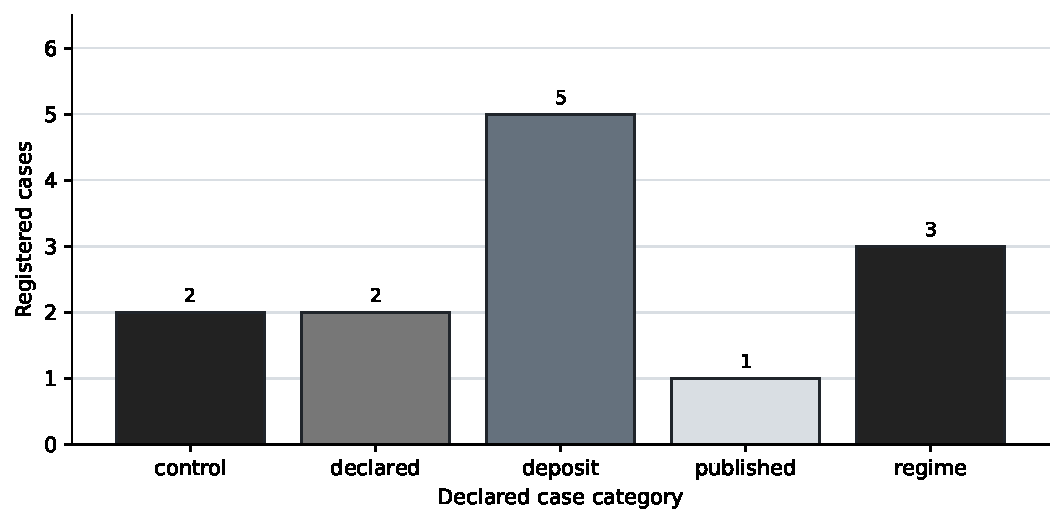
\includegraphics[width=0.82\textwidth]{figures/case-inventory.pdf}\caption{Counts of registered PhaseFlow cases by declared category, derived from the versioned manifest index and limited to this benchmark suite.}\label{fig:case-inventory}\end{figure}
\begin{figure}[htbp]\centering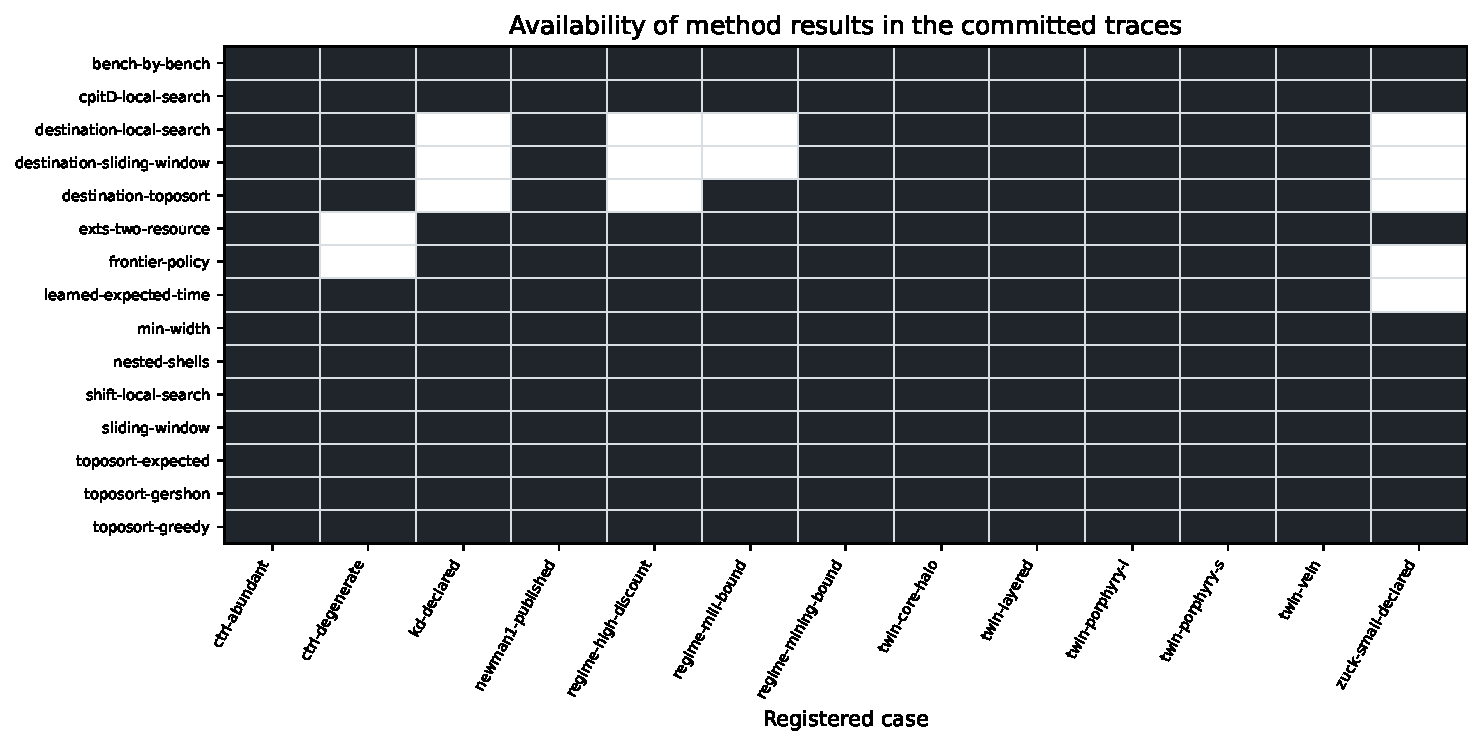
\includegraphics[width=\textwidth]{figures/method-case-coverage.pdf}\caption{Presence of a method result row in each of the thirteen committed traces; a blank cell denotes absent evidence rather than a zero-valued schedule.}\label{fig:method-case-coverage}\end{figure}
\begin{figure}[htbp]\centering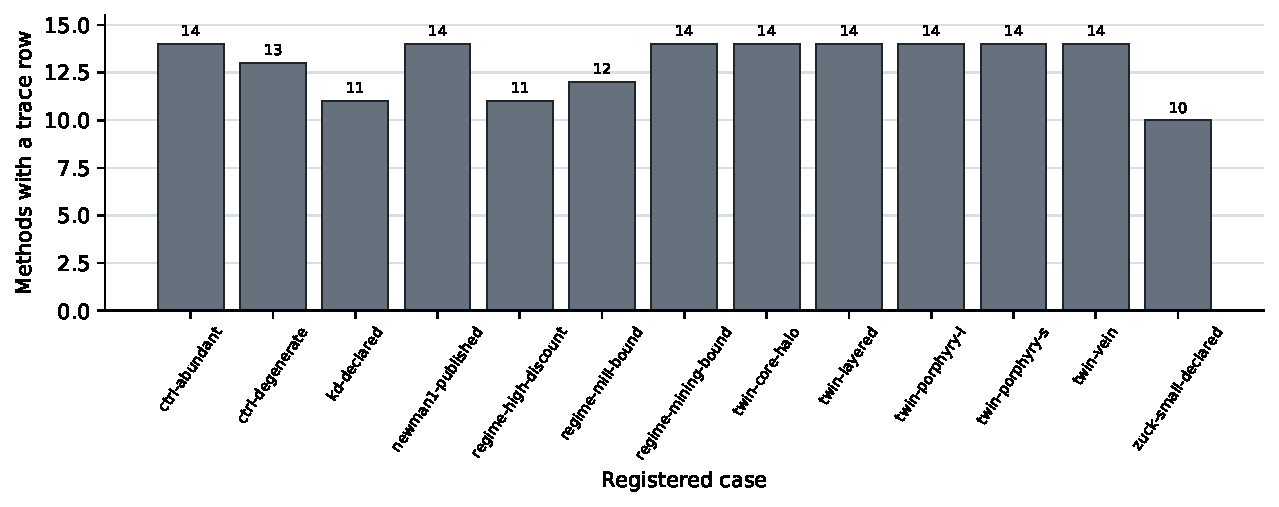
\includegraphics[width=0.9\textwidth]{figures/method-row-counts.pdf}\caption{Number of method rows in every registered case trace, showing where comparisons have different coverage and must not be treated as balanced panels.}\label{fig:method-row-counts}\end{figure}
\begin{figure}[htbp]\centering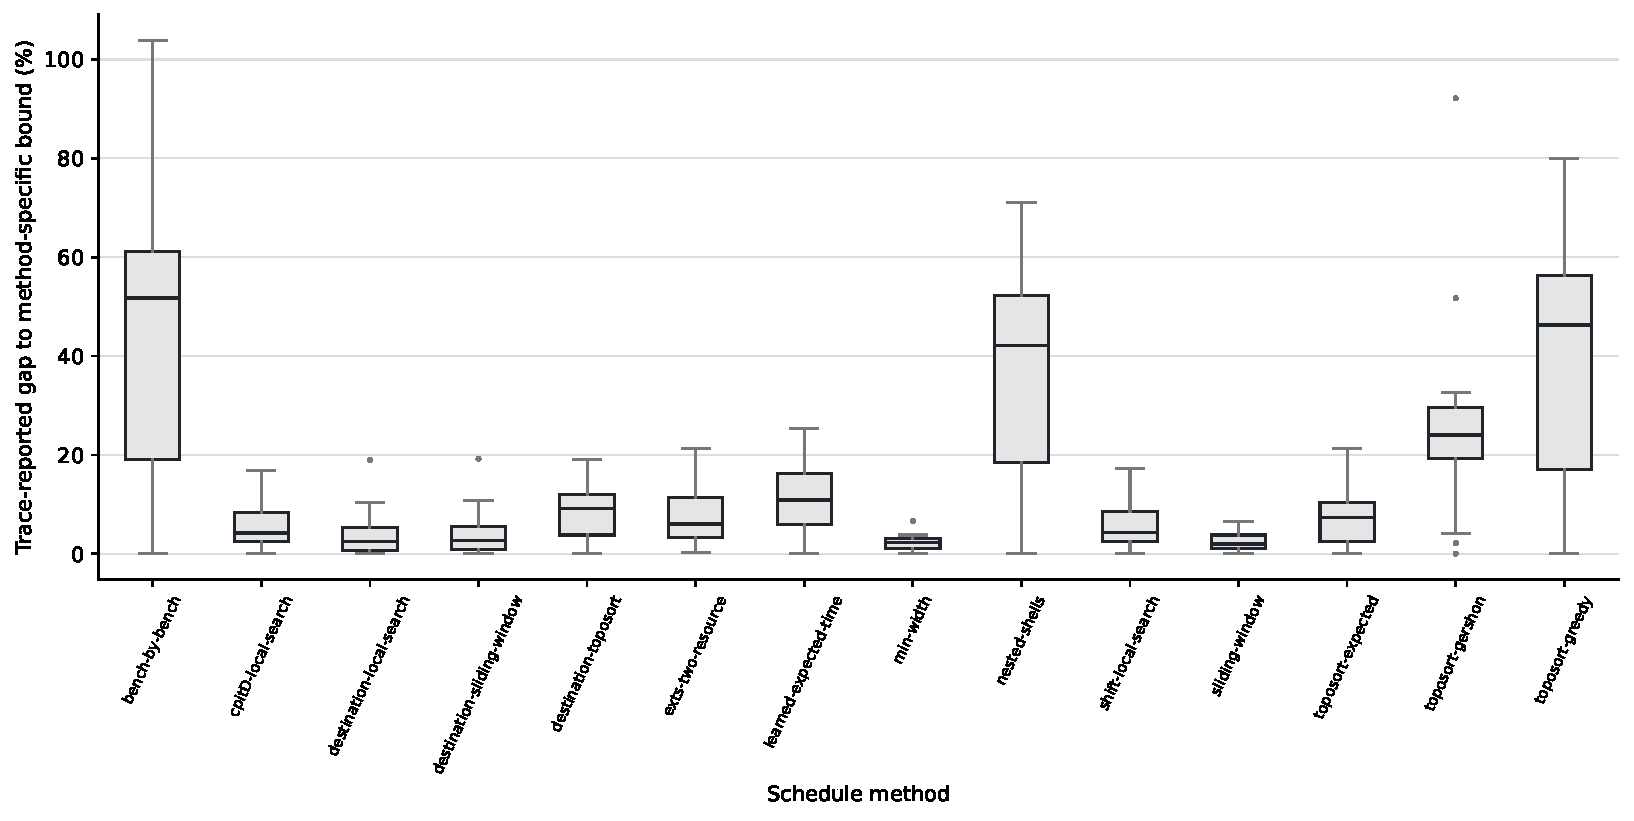
\includegraphics[width=\textwidth]{figures/method-gap-distribution.pdf}\caption{Trace-reported percentage gaps for each method against its own applicable bound across available cases; the plot does not equate distinct formulations.}\label{fig:method-gap-distribution}\end{figure}
\clearpage

The runtime comparison in Figure~\ref{fig:method-runtime} uses wall-clock milliseconds recorded by the pipeline and a logarithmic vertical scale. It shows orders-of-magnitude differences between constructive passes and restricted optimization, but the 13 product cases do not establish asymptotic complexity. Figure~\ref{fig:bound-route-difference} compares the joint and Algorithm 4 bounds only where both are computed. Differences close to zero reflect agreement within the documented column-generation tolerance for those cases; they do not prove that the two routines agree on every CPIT instance. The capacity utilization profile in Figure~\ref{fig:capacity-profile} is from the loose-capacity control and shows period-level use, not a utilization estimate for a mine plan.

Table~\ref{tab:case-method-outcomes} gives the complete case-by-method record from the committed 0.11 benchmark traces. NPV and bound retain each case's source units and should be compared within a case; the gap is the trace-reported percentage and runtime is in milliseconds. Each fixed case-method execution contributes one recorded outcome; repeated runs and inferential uncertainty estimates are unavailable, so the table reports observations rather than confidence intervals. A “no row” entry means the trace emitted no result for that pair and does not mean zero value, infeasibility, or a failed run.

\begingroup\scriptsize\setlength{\tabcolsep}{2.4pt}
\begin{longtable}{>{\raggedright\arraybackslash}p{0.16\textwidth}>{\raggedright\arraybackslash}p{0.25\textwidth}r r r r r}
\caption{Complete recorded outcomes for every registered case and every method observed in the committed 0.11 benchmark traces; missing method rows are shown explicitly and are not imputed.}\label{tab:case-method-outcomes}\\
\toprule Case & Method & Status & \shortstack{NPV\\(case units)} & \shortstack{Bound\\(case units)} & Gap (\%) & Runtime (ms) \\ \midrule\endfirsthead
\toprule Case & Method & Status & \shortstack{NPV\\(case units)} & \shortstack{Bound\\(case units)} & Gap (\%) & Runtime (ms) \\ \midrule\endhead
\texttt{ctrl\allowbreak-abundant} & \texttt{bench\allowbreak-by\allowbreak-bench} & recorded & 398634009.81 & 428750526.53 & 7.0243 & 66.6 \\
\texttt{ctrl\allowbreak-abundant} & \texttt{cpitD\allowbreak-local\allowbreak-search} & recorded & 427644502.81 & 428750526.53 & 0.2580 & 706.0 \\
\texttt{ctrl\allowbreak-abundant} & \texttt{destination\allowbreak-local\allowbreak-search} & recorded & 438028476.84 & 438824758.78 & 0.1815 & 5319.0 \\
\texttt{ctrl\allowbreak-abundant} & \texttt{destination\allowbreak-sliding\allowbreak-window} & recorded & 437899435.07 & 438824758.78 & 0.2109 & 637064.6 \\
\texttt{ctrl\allowbreak-abundant} & \texttt{destination\allowbreak-toposort} & recorded & 437075857.86 & 438824758.78 & 0.3985 & 10335.7 \\
\texttt{ctrl\allowbreak-abundant} & \texttt{exts\allowbreak-two\allowbreak-resource} & recorded & 427325801.23 & 428750526.53 & 0.3323 & 12433.5 \\
\texttt{ctrl\allowbreak-abundant} & \texttt{frontier\allowbreak-policy} & recorded & 413153254.41 & 428750526.53 & 3.6378 & 225500.0 \\
\texttt{ctrl\allowbreak-abundant} & \texttt{learned\allowbreak-expected\allowbreak-time} & recorded & 423393914.47 & 428750526.53 & 1.2494 & 1416.6 \\
\texttt{ctrl\allowbreak-abundant} & \texttt{min\allowbreak-width} & recorded & 427631215.80 & 428750526.53 & 0.2611 & 349.5 \\
\texttt{ctrl\allowbreak-abundant} & \texttt{nested\allowbreak-shells} & recorded & 404889615.93 & 428750526.53 & 5.5652 & 70.3 \\
\texttt{ctrl\allowbreak-abundant} & \texttt{shift\allowbreak-local\allowbreak-search} & recorded & 427637345.93 & 428750526.53 & 0.2596 & 60.1 \\
\texttt{ctrl\allowbreak-abundant} & \texttt{sliding\allowbreak-window} & recorded & 425960870.97 & 428750526.53 & 0.6506 & 234949.2 \\
\texttt{ctrl\allowbreak-abundant} & \texttt{toposort\allowbreak-expected} & recorded & 427325801.23 & 428750526.53 & 0.3323 & 12363.0 \\
\texttt{ctrl\allowbreak-abundant} & \texttt{toposort\allowbreak-gershon} & recorded & 419591568.06 & 428750526.53 & 2.1362 & 195.7 \\
\texttt{ctrl\allowbreak-abundant} & \texttt{toposort\allowbreak-greedy} & recorded & 401470358.50 & 428750526.53 & 6.3627 & 61.7 \\
\texttt{ctrl\allowbreak-degenerate} & \texttt{bench\allowbreak-by\allowbreak-bench} & recorded & 473615065.85 & 473615065.85 & 0.0000 & 87.7 \\
\texttt{ctrl\allowbreak-degenerate} & \texttt{cpitD\allowbreak-local\allowbreak-search} & recorded & 473615065.85 & 473615065.85 & 0.0000 & 338.8 \\
\texttt{ctrl\allowbreak-degenerate} & \texttt{destination\allowbreak-local\allowbreak-search} & recorded & 473615065.85 & 473615065.85 & 0.0000 & 779.6 \\
\texttt{ctrl\allowbreak-degenerate} & \texttt{destination\allowbreak-sliding\allowbreak-window} & recorded & 473615065.85 & 473615065.85 & 0.0000 & 3451.0 \\
\texttt{ctrl\allowbreak-degenerate} & \texttt{destination\allowbreak-toposort} & recorded & 473615065.85 & 473615065.85 & 0.0000 & 523.8 \\
\texttt{ctrl\allowbreak-degenerate} & \texttt{exts\allowbreak-two\allowbreak-resource} & no row & -- & -- & -- & -- \\
\texttt{ctrl\allowbreak-degenerate} & \texttt{frontier\allowbreak-policy} & no row & -- & -- & -- & -- \\
\texttt{ctrl\allowbreak-degenerate} & \texttt{learned\allowbreak-expected\allowbreak-time} & recorded & 473615065.85 & 473615065.85 & 0.0000 & 262.5 \\
\texttt{ctrl\allowbreak-degenerate} & \texttt{min\allowbreak-width} & recorded & 473615065.85 & 473615065.85 & 0.0000 & 334.7 \\
\texttt{ctrl\allowbreak-degenerate} & \texttt{nested\allowbreak-shells} & recorded & 473615065.85 & 473615065.85 & 0.0000 & 78.8 \\
\texttt{ctrl\allowbreak-degenerate} & \texttt{shift\allowbreak-local\allowbreak-search} & recorded & 473615065.85 & 473615065.85 & 0.0000 & 36.3 \\
\texttt{ctrl\allowbreak-degenerate} & \texttt{sliding\allowbreak-window} & recorded & 473615065.85 & 473615065.85 & 0.0000 & 3190.6 \\
\texttt{ctrl\allowbreak-degenerate} & \texttt{toposort\allowbreak-expected} & recorded & 473615065.85 & 473615065.85 & 0.0000 & 393.8 \\
\texttt{ctrl\allowbreak-degenerate} & \texttt{toposort\allowbreak-gershon} & recorded & 473615065.85 & 473615065.85 & 0.0000 & 386.1 \\
\texttt{ctrl\allowbreak-degenerate} & \texttt{toposort\allowbreak-greedy} & recorded & 473615065.85 & 473615065.85 & 0.0000 & 104.5 \\
\texttt{kd\allowbreak-declared} & \texttt{bench\allowbreak-by\allowbreak-bench} & recorded & 161242753.99 & 254345710.51 & 36.6049 & 548.8 \\
\texttt{kd\allowbreak-declared} & \texttt{cpitD\allowbreak-local\allowbreak-search} & recorded & 216143500.33 & 254345710.51 & 15.0198 & 729.9 \\
\texttt{kd\allowbreak-declared} & \texttt{destination\allowbreak-local\allowbreak-search} & no row & -- & -- & -- & -- \\
\texttt{kd\allowbreak-declared} & \texttt{destination\allowbreak-sliding\allowbreak-window} & no row & -- & -- & -- & -- \\
\texttt{kd\allowbreak-declared} & \texttt{destination\allowbreak-toposort} & no row & -- & -- & -- & -- \\
\texttt{kd\allowbreak-declared} & \texttt{exts\allowbreak-two\allowbreak-resource} & recorded & 211382547.37 & 254345710.51 & 16.8916 & 1230282.2 \\
\texttt{kd\allowbreak-declared} & \texttt{frontier\allowbreak-policy} & recorded & 204147475.00 & 254345710.51 & 19.7362 & 747140.0 \\
\texttt{kd\allowbreak-declared} & \texttt{learned\allowbreak-expected\allowbreak-time} & recorded & 189960770.51 & 254345710.51 & 25.3139 & 1003.6 \\
\texttt{kd\allowbreak-declared} & \texttt{min\allowbreak-width} & recorded & 237448230.74 & 254345710.51 & 6.6435 & 377.5 \\
\texttt{kd\allowbreak-declared} & \texttt{nested\allowbreak-shells} & recorded & 162475932.35 & 254345710.51 & 36.1200 & 563.9 \\
\texttt{kd\allowbreak-declared} & \texttt{shift\allowbreak-local\allowbreak-search} & recorded & 215466061.97 & 254345710.51 & 15.2861 & 712.4 \\
\texttt{kd\allowbreak-declared} & \texttt{sliding\allowbreak-window} & recorded & 237922439.65 & 254345710.51 & 6.4571 & 43052723.0 \\
\texttt{kd\allowbreak-declared} & \texttt{toposort\allowbreak-expected} & recorded & 211382547.37 & 254345710.51 & 16.8916 & 1229695.9 \\
\texttt{kd\allowbreak-declared} & \texttt{toposort\allowbreak-gershon} & recorded & 122846659.80 & 254345710.51 & 51.7009 & 1781.6 \\
\texttt{kd\allowbreak-declared} & \texttt{toposort\allowbreak-greedy} & recorded & 173166103.26 & 254345710.51 & 31.9170 & 546.3 \\
\texttt{newman1\allowbreak-published} & \texttt{bench\allowbreak-by\allowbreak-bench} & recorded & 22915556.73 & 24486184.09 & 6.4143 & 10.0 \\
\texttt{newman1\allowbreak-published} & \texttt{cpitD\allowbreak-local\allowbreak-search} & recorded & 23875537.97 & 24486184.09 & 2.4938 & 5370.1 \\
\texttt{newman1\allowbreak-published} & \texttt{destination\allowbreak-local\allowbreak-search} & recorded & 23875640.91 & 24486549.02 & 2.4949 & 16947.4 \\
\texttt{newman1\allowbreak-published} & \texttt{destination\allowbreak-sliding\allowbreak-window} & recorded & 23428618.76 & 24486549.02 & 4.3205 & 19304.9 \\
\texttt{newman1\allowbreak-published} & \texttt{destination\allowbreak-toposort} & recorded & 23864348.55 & 24486549.02 & 2.5410 & 1530.6 \\
\texttt{newman1\allowbreak-published} & \texttt{exts\allowbreak-two\allowbreak-resource} & recorded & 23864348.55 & 24486184.09 & 2.5395 & 2400.7 \\
\texttt{newman1\allowbreak-published} & \texttt{frontier\allowbreak-policy} & recorded & 23054389.44 & 24486184.09 & 5.8474 & 9344.0 \\
\texttt{newman1\allowbreak-published} & \texttt{learned\allowbreak-expected\allowbreak-time} & recorded & 23838465.66 & 24486184.09 & 2.6452 & 42.0 \\
\texttt{newman1\allowbreak-published} & \texttt{min\allowbreak-width} & recorded & 23872009.30 & 24486184.09 & 2.5083 & 54.0 \\
\texttt{newman1\allowbreak-published} & \texttt{nested\allowbreak-shells} & recorded & 23839631.29 & 24486184.09 & 2.6405 & 9.6 \\
\texttt{newman1\allowbreak-published} & \texttt{shift\allowbreak-local\allowbreak-search} & recorded & 23873589.42 & 24486184.09 & 2.5018 & 10.7 \\
\texttt{newman1\allowbreak-published} & \texttt{sliding\allowbreak-window} & recorded & 23428618.76 & 24486184.09 & 4.3190 & 44610.0 \\
\texttt{newman1\allowbreak-published} & \texttt{toposort\allowbreak-expected} & recorded & 23864348.55 & 24486184.09 & 2.5395 & 2390.7 \\
\texttt{newman1\allowbreak-published} & \texttt{toposort\allowbreak-gershon} & recorded & 23474084.43 & 24486184.09 & 4.1333 & 25.1 \\
\texttt{newman1\allowbreak-published} & \texttt{toposort\allowbreak-greedy} & recorded & 23552841.72 & 24486184.09 & 3.8117 & 15.0 \\
\texttt{regime\allowbreak-high\allowbreak-discount} & \texttt{bench\allowbreak-by\allowbreak-bench} & recorded & 71675727.37 & 184634636.79 & 61.1797 & 62.6 \\
\texttt{regime\allowbreak-high\allowbreak-discount} & \texttt{cpitD\allowbreak-local\allowbreak-search} & recorded & 169795008.10 & 184634636.79 & 8.0373 & 970.4 \\
\texttt{regime\allowbreak-high\allowbreak-discount} & \texttt{destination\allowbreak-local\allowbreak-search} & no row & -- & -- & -- & -- \\
\texttt{regime\allowbreak-high\allowbreak-discount} & \texttt{destination\allowbreak-sliding\allowbreak-window} & no row & -- & -- & -- & -- \\
\texttt{regime\allowbreak-high\allowbreak-discount} & \texttt{destination\allowbreak-toposort} & no row & -- & -- & -- & -- \\
\texttt{regime\allowbreak-high\allowbreak-discount} & \texttt{exts\allowbreak-two\allowbreak-resource} & recorded & 168506774.83 & 184634636.79 & 8.7350 & 18649.2 \\
\texttt{regime\allowbreak-high\allowbreak-discount} & \texttt{frontier\allowbreak-policy} & recorded & 159223871.11 & 184634636.79 & 13.7627 & 63328.0 \\
\texttt{regime\allowbreak-high\allowbreak-discount} & \texttt{learned\allowbreak-expected\allowbreak-time} & recorded & 167477586.97 & 184634636.79 & 9.2924 & 10405.9 \\
\texttt{regime\allowbreak-high\allowbreak-discount} & \texttt{min\allowbreak-width} & recorded & 181077135.78 & 184634636.79 & 1.9268 & 1172.4 \\
\texttt{regime\allowbreak-high\allowbreak-discount} & \texttt{nested\allowbreak-shells} & recorded & 88065737.46 & 184634636.79 & 52.3027 & 60.9 \\
\texttt{regime\allowbreak-high\allowbreak-discount} & \texttt{shift\allowbreak-local\allowbreak-search} & recorded & 169738335.86 & 184634636.79 & 8.0680 & 43.1 \\
\texttt{regime\allowbreak-high\allowbreak-discount} & \texttt{sliding\allowbreak-window} & recorded & 181093517.32 & 184634636.79 & 1.9179 & 870157.4 \\
\texttt{regime\allowbreak-high\allowbreak-discount} & \texttt{toposort\allowbreak-expected} & recorded & 168506774.83 & 184634636.79 & 8.7350 & 18586.7 \\
\texttt{regime\allowbreak-high\allowbreak-discount} & \texttt{toposort\allowbreak-gershon} & recorded & 141804901.67 & 184634636.79 & 23.1970 & 182.1 \\
\texttt{regime\allowbreak-high\allowbreak-discount} & \texttt{toposort\allowbreak-greedy} & recorded & 80712545.33 & 184634636.79 & 56.2853 & 61.1 \\
\texttt{regime\allowbreak-mill\allowbreak-bound} & \texttt{bench\allowbreak-by\allowbreak-bench} & recorded & 27438402.44 & 129686447.19 & 78.8425 & 112.1 \\
\texttt{regime\allowbreak-mill\allowbreak-bound} & \texttt{cpitD\allowbreak-local\allowbreak-search} & recorded & 112011241.62 & 129686447.19 & 13.6292 & 3957.9 \\
\texttt{regime\allowbreak-mill\allowbreak-bound} & \texttt{destination\allowbreak-local\allowbreak-search} & no row & -- & -- & -- & -- \\
\texttt{regime\allowbreak-mill\allowbreak-bound} & \texttt{destination\allowbreak-sliding\allowbreak-window} & no row & -- & -- & -- & -- \\
\texttt{regime\allowbreak-mill\allowbreak-bound} & \texttt{destination\allowbreak-toposort} & recorded & 190273768.14 & 207638996.94 & 8.3632 & 76867.0 \\
\texttt{regime\allowbreak-mill\allowbreak-bound} & \texttt{exts\allowbreak-two\allowbreak-resource} & recorded & 110317470.62 & 129686447.19 & 14.9352 & 37493.1 \\
\texttt{regime\allowbreak-mill\allowbreak-bound} & \texttt{frontier\allowbreak-policy} & recorded & 101124141.73 & 129686447.19 & 22.0241 & 41891.0 \\
\texttt{regime\allowbreak-mill\allowbreak-bound} & \texttt{learned\allowbreak-expected\allowbreak-time} & recorded & 112281367.00 & 129686447.19 & 13.4209 & 339.1 \\
\texttt{regime\allowbreak-mill\allowbreak-bound} & \texttt{min\allowbreak-width} & recorded & 124764860.94 & 129686447.19 & 3.7950 & 117.8 \\
\texttt{regime\allowbreak-mill\allowbreak-bound} & \texttt{nested\allowbreak-shells} & recorded & 37413390.52 & 129686447.19 & 71.1509 & 107.9 \\
\texttt{regime\allowbreak-mill\allowbreak-bound} & \texttt{shift\allowbreak-local\allowbreak-search} & recorded & 111801028.46 & 129686447.19 & 13.7913 & 68.3 \\
\texttt{regime\allowbreak-mill\allowbreak-bound} & \texttt{sliding\allowbreak-window} & recorded & 124764198.75 & 129686447.19 & 3.7955 & 8094593.2 \\
\texttt{regime\allowbreak-mill\allowbreak-bound} & \texttt{toposort\allowbreak-expected} & recorded & 110317470.62 & 129686447.19 & 14.9352 & 37373.2 \\
\texttt{regime\allowbreak-mill\allowbreak-bound} & \texttt{toposort\allowbreak-gershon} & recorded & 91229398.23 & 129686447.19 & 29.6539 & 423.3 \\
\texttt{regime\allowbreak-mill\allowbreak-bound} & \texttt{toposort\allowbreak-greedy} & recorded & 37580828.14 & 129686447.19 & 71.0218 & 97.1 \\
\texttt{regime\allowbreak-mining\allowbreak-bound} & \texttt{bench\allowbreak-by\allowbreak-bench} & recorded & 46282695.39 & 187991036.34 & 75.3804 & 97.8 \\
\texttt{regime\allowbreak-mining\allowbreak-bound} & \texttt{cpitD\allowbreak-local\allowbreak-search} & recorded & 173959432.24 & 187991036.34 & 7.4640 & 1354.4 \\
\texttt{regime\allowbreak-mining\allowbreak-bound} & \texttt{destination\allowbreak-local\allowbreak-search} & recorded & 182965952.37 & 187991036.34 & 2.6730 & 2547.9 \\
\texttt{regime\allowbreak-mining\allowbreak-bound} & \texttt{destination\allowbreak-sliding\allowbreak-window} & recorded & 182955948.65 & 187991036.34 & 2.6784 & 293727.3 \\
\texttt{regime\allowbreak-mining\allowbreak-bound} & \texttt{destination\allowbreak-toposort} & recorded & 173833944.80 & 187991036.34 & 7.5307 & 33821.0 \\
\texttt{regime\allowbreak-mining\allowbreak-bound} & \texttt{exts\allowbreak-two\allowbreak-resource} & recorded & 173936547.76 & 187991036.34 & 7.4761 & 27157.4 \\
\texttt{regime\allowbreak-mining\allowbreak-bound} & \texttt{frontier\allowbreak-policy} & recorded & 136789708.76 & 187991036.34 & 27.2360 & 52953.0 \\
\texttt{regime\allowbreak-mining\allowbreak-bound} & \texttt{learned\allowbreak-expected\allowbreak-time} & recorded & 165775509.75 & 187991036.34 & 11.8173 & 250.9 \\
\texttt{regime\allowbreak-mining\allowbreak-bound} & \texttt{min\allowbreak-width} & recorded & 182955948.65 & 187991036.34 & 2.6784 & 104.5 \\
\texttt{regime\allowbreak-mining\allowbreak-bound} & \texttt{nested\allowbreak-shells} & recorded & 84693368.98 & 187991036.34 & 54.9482 & 91.6 \\
\texttt{regime\allowbreak-mining\allowbreak-bound} & \texttt{shift\allowbreak-local\allowbreak-search} & recorded & 173936547.76 & 187991036.34 & 7.4761 & 48.7 \\
\texttt{regime\allowbreak-mining\allowbreak-bound} & \texttt{sliding\allowbreak-window} & recorded & 182955948.65 & 187991036.34 & 2.6784 & 414483.6 \\
\texttt{regime\allowbreak-mining\allowbreak-bound} & \texttt{toposort\allowbreak-expected} & recorded & 173833944.80 & 187991036.34 & 7.5307 & 27070.9 \\
\texttt{regime\allowbreak-mining\allowbreak-bound} & \texttt{toposort\allowbreak-gershon} & recorded & 135904818.17 & 187991036.34 & 27.7068 & 344.4 \\
\texttt{regime\allowbreak-mining\allowbreak-bound} & \texttt{toposort\allowbreak-greedy} & recorded & 80886097.28 & 187991036.34 & 56.9734 & 85.4 \\
\texttt{twin\allowbreak-core\allowbreak-halo} & \texttt{bench\allowbreak-by\allowbreak-bench} & recorded & -3749944.12 & 97374025.65 & 103.8511 & 119.9 \\
\texttt{twin\allowbreak-core\allowbreak-halo} & \texttt{cpitD\allowbreak-local\allowbreak-search} & recorded & 89185799.33 & 97374025.65 & 8.4090 & 375.4 \\
\texttt{twin\allowbreak-core\allowbreak-halo} & \texttt{destination\allowbreak-local\allowbreak-search} & recorded & 124888369.55 & 131860391.69 & 5.2874 & 2017.0 \\
\texttt{twin\allowbreak-core\allowbreak-halo} & \texttt{destination\allowbreak-sliding\allowbreak-window} & recorded & 124663891.68 & 131860391.69 & 5.4577 & 100898440.8 \\
\texttt{twin\allowbreak-core\allowbreak-halo} & \texttt{destination\allowbreak-toposort} & recorded & 110093184.62 & 131860391.69 & 16.5078 & 193498.5 \\
\texttt{twin\allowbreak-core\allowbreak-halo} & \texttt{exts\allowbreak-two\allowbreak-resource} & recorded & 87353942.61 & 97374025.65 & 10.2903 & 38870.5 \\
\texttt{twin\allowbreak-core\allowbreak-halo} & \texttt{frontier\allowbreak-policy} & recorded & 12960635.64 & 97374025.65 & 86.6898 & 240375.0 \\
\texttt{twin\allowbreak-core\allowbreak-halo} & \texttt{learned\allowbreak-expected\allowbreak-time} & recorded & 76238349.72 & 97374025.65 & 21.7057 & 306.0 \\
\texttt{twin\allowbreak-core\allowbreak-halo} & \texttt{min\allowbreak-width} & recorded & 94383318.02 & 97374025.65 & 3.0714 & 333.8 \\
\texttt{twin\allowbreak-core\allowbreak-halo} & \texttt{nested\allowbreak-shells} & recorded & 32082724.70 & 97374025.65 & 67.0521 & 120.2 \\
\texttt{twin\allowbreak-core\allowbreak-halo} & \texttt{shift\allowbreak-local\allowbreak-search} & recorded & 89079079.40 & 97374025.65 & 8.5186 & 80.2 \\
\texttt{twin\allowbreak-core\allowbreak-halo} & \texttt{sliding\allowbreak-window} & recorded & 94400395.06 & 97374025.65 & 3.0538 & 4427029.4 \\
\texttt{twin\allowbreak-core\allowbreak-halo} & \texttt{toposort\allowbreak-expected} & recorded & 87353942.61 & 97374025.65 & 10.2903 & 38764.5 \\
\texttt{twin\allowbreak-core\allowbreak-halo} & \texttt{toposort\allowbreak-gershon} & recorded & 72931998.92 & 97374025.65 & 25.1012 & 431.6 \\
\texttt{twin\allowbreak-core\allowbreak-halo} & \texttt{toposort\allowbreak-greedy} & recorded & 19478724.49 & 97374025.65 & 79.9960 & 111.5 \\
\texttt{twin\allowbreak-layered} & \texttt{bench\allowbreak-by\allowbreak-bench} & recorded & 899817035.61 & 1111128368.75 & 19.0177 & 278.3 \\
\texttt{twin\allowbreak-layered} & \texttt{cpitD\allowbreak-local\allowbreak-search} & recorded & 1071699060.76 & 1111128368.75 & 3.5486 & 1504.3 \\
\texttt{twin\allowbreak-layered} & \texttt{destination\allowbreak-local\allowbreak-search} & recorded & 1223250861.55 & 1365530202.41 & 10.4193 & 15999.8 \\
\texttt{twin\allowbreak-layered} & \texttt{destination\allowbreak-sliding\allowbreak-window} & recorded & 1218078182.62 & 1365530202.41 & 10.7982 & 26903036.2 \\
\texttt{twin\allowbreak-layered} & \texttt{destination\allowbreak-toposort} & recorded & 1199918922.00 & 1365530202.41 & 12.1280 & 102246.9 \\
\texttt{twin\allowbreak-layered} & \texttt{exts\allowbreak-two\allowbreak-resource} & recorded & 1071675842.38 & 1111128368.75 & 3.5507 & 142978.2 \\
\texttt{twin\allowbreak-layered} & \texttt{frontier\allowbreak-policy} & recorded & 954631473.15 & 1111128368.75 & 14.0845 & 337594.0 \\
\texttt{twin\allowbreak-layered} & \texttt{learned\allowbreak-expected\allowbreak-time} & recorded & 943692071.51 & 1111128368.75 & 15.0690 & 467.2 \\
\texttt{twin\allowbreak-layered} & \texttt{min\allowbreak-width} & recorded & 1071699060.76 & 1111128368.75 & 3.5486 & 483.0 \\
\texttt{twin\allowbreak-layered} & \texttt{nested\allowbreak-shells} & recorded & 906350214.91 & 1111128368.75 & 18.4297 & 268.5 \\
\texttt{twin\allowbreak-layered} & \texttt{shift\allowbreak-local\allowbreak-search} & recorded & 1071675842.38 & 1111128368.75 & 3.5507 & 125.8 \\
\texttt{twin\allowbreak-layered} & \texttt{sliding\allowbreak-window} & recorded & 1043154180.50 & 1111128368.75 & 6.1176 & 61319696.8 \\
\texttt{twin\allowbreak-layered} & \texttt{toposort\allowbreak-expected} & recorded & 1071675842.38 & 1111128368.75 & 3.5507 & 142672.4 \\
\texttt{twin\allowbreak-layered} & \texttt{toposort\allowbreak-gershon} & recorded & 896014135.91 & 1111128368.75 & 19.3600 & 960.3 \\
\texttt{twin\allowbreak-layered} & \texttt{toposort\allowbreak-greedy} & recorded & 922170648.98 & 1111128368.75 & 17.0059 & 266.9 \\
\texttt{twin\allowbreak-porphyry\allowbreak-l} & \texttt{bench\allowbreak-by\allowbreak-bench} & recorded & 130457207.30 & 326536184.81 & 60.0482 & 152.7 \\
\texttt{twin\allowbreak-porphyry\allowbreak-l} & \texttt{cpitD\allowbreak-local\allowbreak-search} & recorded & 314277464.74 & 326536184.81 & 3.7542 & 554.6 \\
\texttt{twin\allowbreak-porphyry\allowbreak-l} & \texttt{destination\allowbreak-local\allowbreak-search} & recorded & 435284799.50 & 442009362.99 & 1.5214 & 2520.4 \\
\texttt{twin\allowbreak-porphyry\allowbreak-l} & \texttt{destination\allowbreak-sliding\allowbreak-window} & recorded & 434585393.36 & 442009362.99 & 1.6796 & 7597200.9 \\
\texttt{twin\allowbreak-porphyry\allowbreak-l} & \texttt{destination\allowbreak-toposort} & recorded & 391770770.21 & 442009362.99 & 11.3660 & 112771.1 \\
\texttt{twin\allowbreak-porphyry\allowbreak-l} & \texttt{exts\allowbreak-two\allowbreak-resource} & recorded & 312945549.84 & 326536184.81 & 4.1621 & 93434.3 \\
\texttt{twin\allowbreak-porphyry\allowbreak-l} & \texttt{frontier\allowbreak-policy} & recorded & 277296868.19 & 326536184.81 & 15.0793 & 140468.0 \\
\texttt{twin\allowbreak-porphyry\allowbreak-l} & \texttt{learned\allowbreak-expected\allowbreak-time} & recorded & 294357112.95 & 326536184.81 & 9.8547 & 227.6 \\
\texttt{twin\allowbreak-porphyry\allowbreak-l} & \texttt{min\allowbreak-width} & recorded & 321364047.29 & 326536184.81 & 1.5839 & 399.9 \\
\texttt{twin\allowbreak-porphyry\allowbreak-l} & \texttt{nested\allowbreak-shells} & recorded & 178634640.63 & 326536184.81 & 45.2941 & 142.8 \\
\texttt{twin\allowbreak-porphyry\allowbreak-l} & \texttt{shift\allowbreak-local\allowbreak-search} & recorded & 314247297.94 & 326536184.81 & 3.7634 & 107.6 \\
\texttt{twin\allowbreak-porphyry\allowbreak-l} & \texttt{sliding\allowbreak-window} & recorded & 321380848.23 & 326536184.81 & 1.5788 & 8228931.2 \\
\texttt{twin\allowbreak-porphyry\allowbreak-l} & \texttt{toposort\allowbreak-expected} & recorded & 302668911.25 & 326536184.81 & 7.3092 & 93282.8 \\
\texttt{twin\allowbreak-porphyry\allowbreak-l} & \texttt{toposort\allowbreak-gershon} & recorded & 248020634.26 & 326536184.81 & 24.0450 & 571.2 \\
\texttt{twin\allowbreak-porphyry\allowbreak-l} & \texttt{toposort\allowbreak-greedy} & recorded & 168760440.49 & 326536184.81 & 48.3180 & 144.8 \\
\texttt{twin\allowbreak-porphyry\allowbreak-s} & \texttt{bench\allowbreak-by\allowbreak-bench} & recorded & 107531529.28 & 234230541.78 & 54.0916 & 93.2 \\
\texttt{twin\allowbreak-porphyry\allowbreak-s} & \texttt{cpitD\allowbreak-local\allowbreak-search} & recorded & 224340746.28 & 234230541.78 & 4.2222 & 966.0 \\
\texttt{twin\allowbreak-porphyry\allowbreak-s} & \texttt{destination\allowbreak-local\allowbreak-search} & recorded & 314279336.50 & 316475407.00 & 0.6939 & 1198.4 \\
\texttt{twin\allowbreak-porphyry\allowbreak-s} & \texttt{destination\allowbreak-sliding\allowbreak-window} & recorded & 314005925.57 & 316475407.00 & 0.7803 & 5247976.1 \\
\texttt{twin\allowbreak-porphyry\allowbreak-s} & \texttt{destination\allowbreak-toposort} & recorded & 285163568.34 & 316475407.00 & 9.8939 & 54428.5 \\
\texttt{twin\allowbreak-porphyry\allowbreak-s} & \texttt{exts\allowbreak-two\allowbreak-resource} & recorded & 223413684.70 & 234230541.78 & 4.6180 & 28809.3 \\
\texttt{twin\allowbreak-porphyry\allowbreak-s} & \texttt{frontier\allowbreak-policy} & recorded & 209106102.27 & 234230541.78 & 10.7264 & 66593.0 \\
\texttt{twin\allowbreak-porphyry\allowbreak-s} & \texttt{learned\allowbreak-expected\allowbreak-time} & recorded & 217707634.04 & 234230541.78 & 7.0541 & 158.8 \\
\texttt{twin\allowbreak-porphyry\allowbreak-s} & \texttt{min\allowbreak-width} & recorded & 231603547.81 & 234230541.78 & 1.1215 & 128.0 \\
\texttt{twin\allowbreak-porphyry\allowbreak-s} & \texttt{nested\allowbreak-shells} & recorded & 130810346.26 & 234230541.78 & 44.1532 & 87.4 \\
\texttt{twin\allowbreak-porphyry\allowbreak-s} & \texttt{shift\allowbreak-local\allowbreak-search} & recorded & 224241882.03 & 234230541.78 & 4.2645 & 54.3 \\
\texttt{twin\allowbreak-porphyry\allowbreak-s} & \texttt{sliding\allowbreak-window} & recorded & 231622561.26 & 234230541.78 & 1.1134 & 3166607.9 \\
\texttt{twin\allowbreak-porphyry\allowbreak-s} & \texttt{toposort\allowbreak-expected} & recorded & 223413684.70 & 234230541.78 & 4.6180 & 28726.8 \\
\texttt{twin\allowbreak-porphyry\allowbreak-s} & \texttt{toposort\allowbreak-gershon} & recorded & 187236534.51 & 234230541.78 & 20.0631 & 299.7 \\
\texttt{twin\allowbreak-porphyry\allowbreak-s} & \texttt{toposort\allowbreak-greedy} & recorded & 117596777.73 & 234230541.78 & 49.7944 & 80.9 \\
\texttt{twin\allowbreak-vein} & \texttt{bench\allowbreak-by\allowbreak-bench} & recorded & 172734791.93 & 285385073.56 & 39.4731 & 231.7 \\
\texttt{twin\allowbreak-vein} & \texttt{cpitD\allowbreak-local\allowbreak-search} & recorded & 283628430.36 & 285385073.56 & 0.6155 & 985.4 \\
\texttt{twin\allowbreak-vein} & \texttt{destination\allowbreak-local\allowbreak-search} & recorded & 300153975.44 & 370316500.73 & 18.9466 & 8967.0 \\
\texttt{twin\allowbreak-vein} & \texttt{destination\allowbreak-sliding\allowbreak-window} & recorded & 299142002.02 & 370316500.73 & 19.2199 & 3689975.7 \\
\texttt{twin\allowbreak-vein} & \texttt{destination\allowbreak-toposort} & recorded & 299979371.52 & 370316500.73 & 18.9938 & 357718.2 \\
\texttt{twin\allowbreak-vein} & \texttt{exts\allowbreak-two\allowbreak-resource} & recorded & 280993395.08 & 285385073.56 & 1.5389 & 93610.0 \\
\texttt{twin\allowbreak-vein} & \texttt{frontier\allowbreak-policy} & recorded & 223609743.51 & 285385073.56 & 21.6463 & 220563.0 \\
\texttt{twin\allowbreak-vein} & \texttt{learned\allowbreak-expected\allowbreak-time} & recorded & 229200036.05 & 285385073.56 & 19.6874 & 407.9 \\
\texttt{twin\allowbreak-vein} & \texttt{min\allowbreak-width} & recorded & 285102255.15 & 285385073.56 & 0.0991 & 690.8 \\
\texttt{twin\allowbreak-vein} & \texttt{nested\allowbreak-shells} & recorded & 165147496.81 & 285385073.56 & 42.1317 & 222.7 \\
\texttt{twin\allowbreak-vein} & \texttt{shift\allowbreak-local\allowbreak-search} & recorded & 283568073.89 & 285385073.56 & 0.6367 & 147.9 \\
\texttt{twin\allowbreak-vein} & \texttt{sliding\allowbreak-window} & recorded & 285108029.53 & 285385073.56 & 0.0971 & 2062209.0 \\
\texttt{twin\allowbreak-vein} & \texttt{toposort\allowbreak-expected} & recorded & 280993395.08 & 285385073.56 & 1.5389 & 93387.5 \\
\texttt{twin\allowbreak-vein} & \texttt{toposort\allowbreak-gershon} & recorded & 22428664.26 & 285385073.56 & 92.1409 & 1024.9 \\
\texttt{twin\allowbreak-vein} & \texttt{toposort\allowbreak-greedy} & recorded & 181068401.86 & 285385073.56 & 36.5530 & 217.9 \\
\texttt{zuck\allowbreak-small\allowbreak-declared} & \texttt{bench\allowbreak-by\allowbreak-bench} & recorded & 346832457.33 & 719234226.20 & 51.7775 & 276.7 \\
\texttt{zuck\allowbreak-small\allowbreak-declared} & \texttt{cpitD\allowbreak-local\allowbreak-search} & recorded & 597620803.33 & 719234226.20 & 16.9087 & 454.1 \\
\texttt{zuck\allowbreak-small\allowbreak-declared} & \texttt{destination\allowbreak-local\allowbreak-search} & no row & -- & -- & -- & -- \\
\texttt{zuck\allowbreak-small\allowbreak-declared} & \texttt{destination\allowbreak-sliding\allowbreak-window} & no row & -- & -- & -- & -- \\
\texttt{zuck\allowbreak-small\allowbreak-declared} & \texttt{destination\allowbreak-toposort} & no row & -- & -- & -- & -- \\
\texttt{zuck\allowbreak-small\allowbreak-declared} & \texttt{exts\allowbreak-two\allowbreak-resource} & recorded & 566520496.41 & 719234226.20 & 21.2328 & 254238.3 \\
\texttt{zuck\allowbreak-small\allowbreak-declared} & \texttt{frontier\allowbreak-policy} & no row & -- & -- & -- & -- \\
\texttt{zuck\allowbreak-small\allowbreak-declared} & \texttt{learned\allowbreak-expected\allowbreak-time} & no row & -- & -- & -- & -- \\
\texttt{zuck\allowbreak-small\allowbreak-declared} & \texttt{min\allowbreak-width} & recorded & 703210120.67 & 719234226.20 & 2.2279 & 314.5 \\
\texttt{zuck\allowbreak-small\allowbreak-declared} & \texttt{nested\allowbreak-shells} & recorded & 495393569.72 & 719234226.20 & 31.1221 & 256.9 \\
\texttt{zuck\allowbreak-small\allowbreak-declared} & \texttt{shift\allowbreak-local\allowbreak-search} & recorded & 594985768.04 & 719234226.20 & 17.2751 & 427.3 \\
\texttt{zuck\allowbreak-small\allowbreak-declared} & \texttt{sliding\allowbreak-window} & recorded & 705009489.02 & 719234226.20 & 1.9778 & 6579257.9 \\
\texttt{zuck\allowbreak-small\allowbreak-declared} & \texttt{toposort\allowbreak-expected} & recorded & 565706313.09 & 719234226.20 & 21.3460 & 253978.8 \\
\texttt{zuck\allowbreak-small\allowbreak-declared} & \texttt{toposort\allowbreak-gershon} & recorded & 483991842.71 & 719234226.20 & 32.7073 & 735.6 \\
\texttt{zuck\allowbreak-small\allowbreak-declared} & \texttt{toposort\allowbreak-greedy} & recorded & 386377893.10 & 719234226.20 & 46.2793 & 249.7 \\
\bottomrule\end{longtable}\endgroup

\clearpage

\begin{figure}[htbp]\centering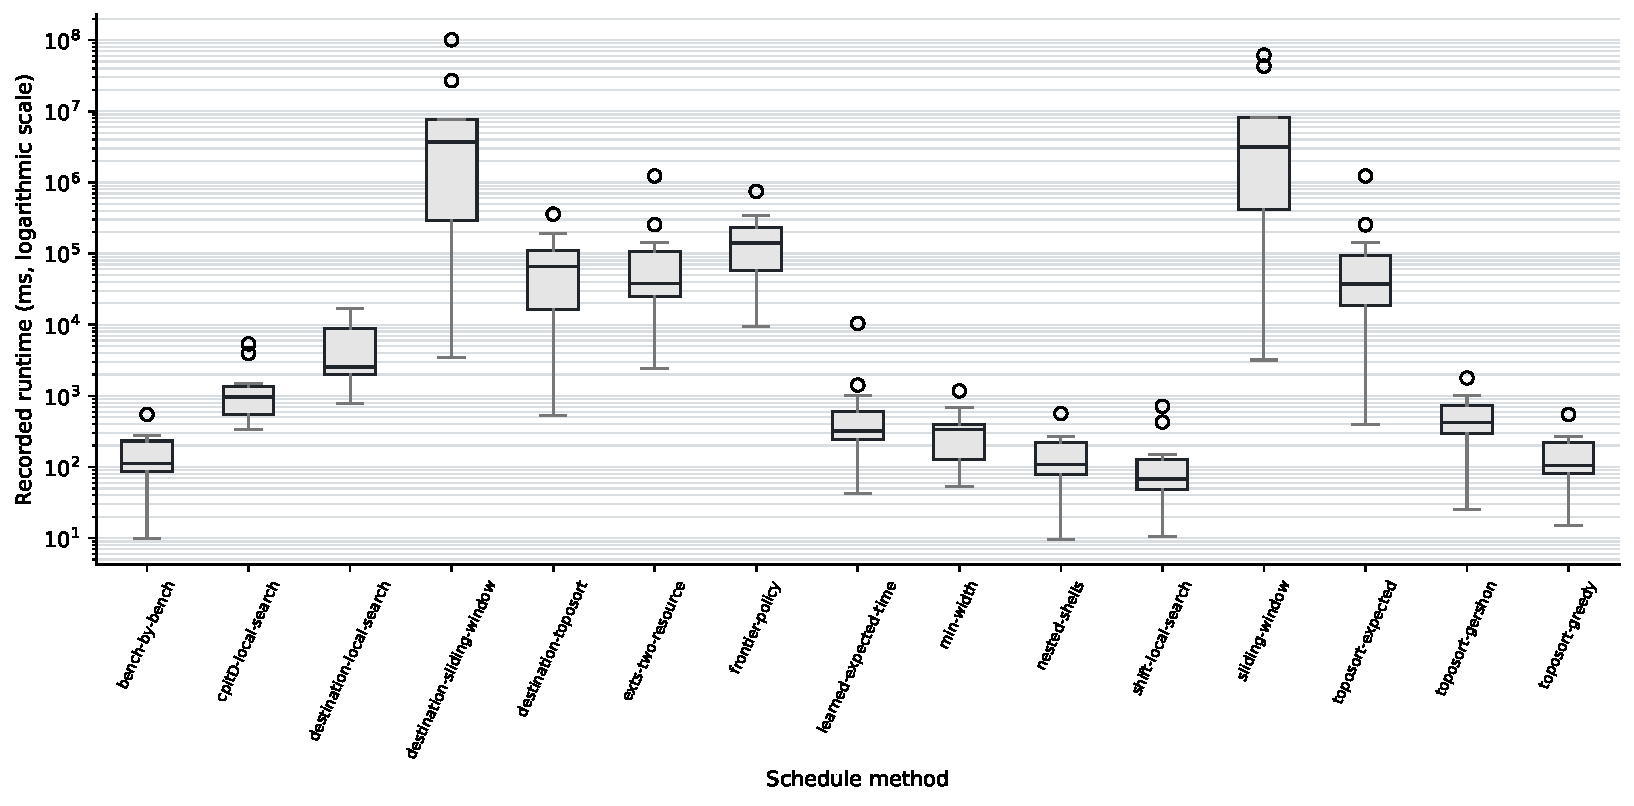
\includegraphics[width=\textwidth]{figures/method-runtime.pdf}\caption{Recorded runtime distributions by schedule method over the cases that contain a runtime, with logarithmic scaling preserving both short constructive passes and long optimization runs.}\label{fig:method-runtime}\end{figure}
\begin{figure}[htbp]\centering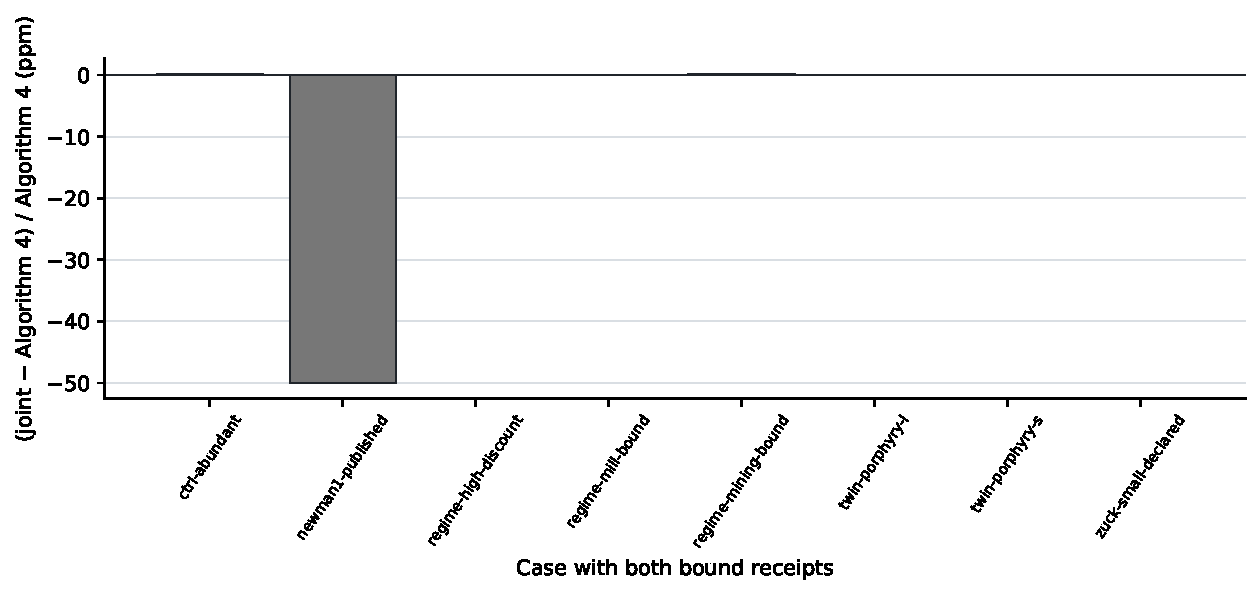
\includegraphics[width=0.82\textwidth]{figures/bound-route-difference.pdf}\caption{Relative difference in parts per million between two upper-bound computations on cases where both are present, retaining the sign and the bound provenance.}\label{fig:bound-route-difference}\end{figure}
\begin{figure}[htbp]\centering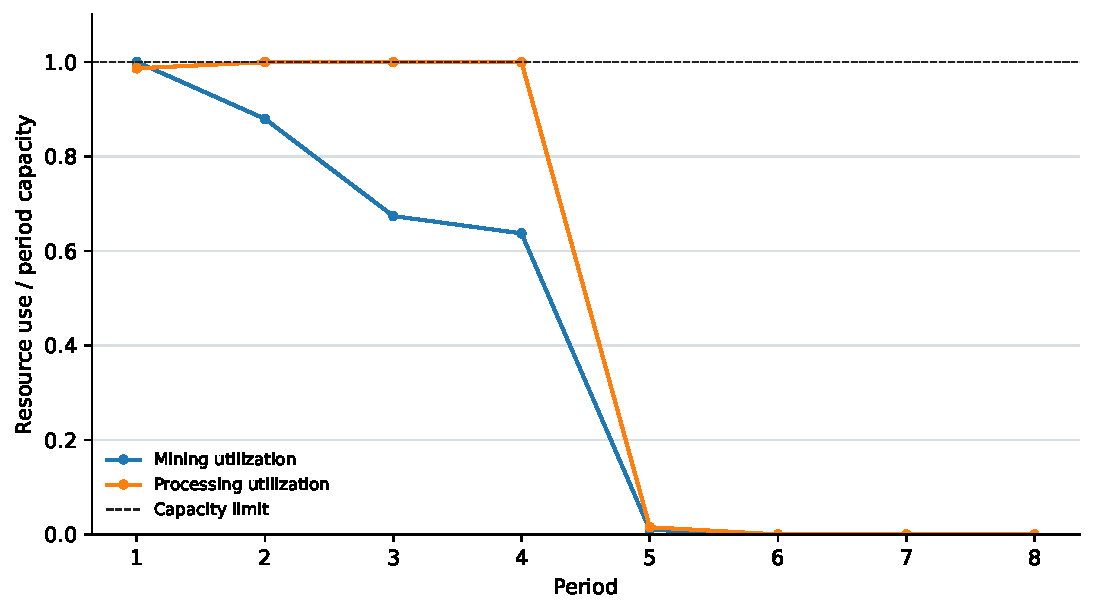
\includegraphics[width=0.82\textwidth]{figures/capacity-profile.pdf}\caption{Period resource utilization for the declared loose-capacity diagnostic, calculated from the selected trace's mined tonnes and resource limits.}\label{fig:capacity-profile}\end{figure}
\clearpage

Table~\ref{tab:method-result-summary} is the trace-level detail behind the method coverage and runtime summaries: the
available row count ranges from 9 to 13 cases, and the destination sliding-window trace reaches 100,898,440.8 ms,
compared with 548.8 ms for the bench-by-bench constructor. These are observed runtimes on this fixed suite, not
complexity estimates. Because the methods have different formulations and the table uses only traces that contain a
row, its medians describe availability-conditioned results and do not support a single cross-method ranking.
\begingroup\small\setlength{\tabcolsep}{3pt}
\begin{longtable}{>{\raggedright\arraybackslash}p{0.34\textwidth}rrrr}
\caption{Registered case traces report method-specific gaps and runtimes; absent rows are not imputed as zero.}\label{tab:method-summary}\\
\toprule Method & Cases & Median gap (\%) & Median ms & Maximum ms \\ \midrule\endfirsthead
\toprule Method & Cases & Median gap (\%) & Median ms & Maximum ms \\ \midrule\endhead
\path{bench-by-bench} & 13 & 51.7775 & 112.1 & 548.8 \\
\path{cpitD-local-search} & 13 & 4.2222 & 966.0 & 5370.1 \\
\path{destination-local-search} & 9 & 2.4949 & 2547.9 & 16947.4 \\
\path{destination-sliding-window} & 9 & 2.6784 & 3689975.7 & 100898440.8 \\
\path{destination-toposort} & 10 & 9.1286 & 65647.8 & 357718.2 \\
\path{exts-two-resource} & 12 & 6.0471 & 38181.8 & 1230282.2 \\
\path{learned-expected-time} & 12 & 10.8360 & 322.6 & 10405.9 \\
\path{min-width} & 13 & 2.2279 & 334.7 & 1172.4 \\
\path{nested-shells} & 13 & 42.1317 & 107.9 & 563.9 \\
\path{shift-local-search} & 13 & 4.2645 & 68.3 & 712.4 \\
\path{sliding-window} & 13 & 1.9778 & 3166607.9 & 61319696.8 \\
\path{toposort-expected} & 13 & 7.3092 & 37373.2 & 1229695.9 \\
\path{toposort-gershon} & 13 & 24.0450 & 423.3 & 1781.6 \\
\path{toposort-greedy} & 13 & 46.2793 & 104.5 & 546.3 \\
\bottomrule\end{longtable}\endgroup


\subsection{Learned expected-time results and failure analysis}
The deposit-disjoint synthetic holdout is summarized by archetype in Figure~\ref{fig:learned-holdout-by-archetype} and Table~\ref{tab:learned-by-archetype}. The median, lower quantiles, and individual minima differ materially by family; the aggregate median of 0.9405 therefore hides a weak tail. The figure describes four generated families under the fixed design, not a probability distribution over real deposits. Figure~\ref{fig:learned-failure-rate} gives the fraction of held-out cases below the 0.90 diagnostic ratio, computed from the same 432 rows. The diagnostic threshold is study-specific and does not constitute an operational acceptance threshold.

\begin{figure}[htbp]\centering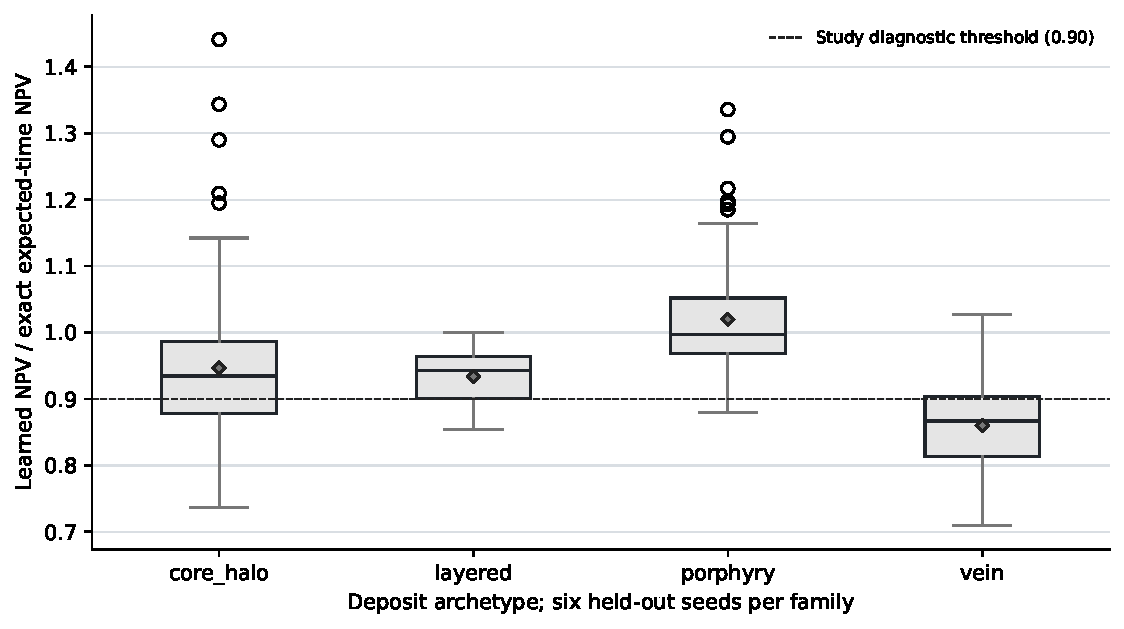
\includegraphics[width=0.86\textwidth]{figures/learned-holdout-by-archetype.pdf}\caption{Distribution of learned-to-exact expected-time schedule value over deposit-disjoint holdout cases, grouped by four generated archetypes and marked at the study threshold.}\label{fig:learned-holdout-by-archetype}\end{figure}
\begin{figure}[htbp]\centering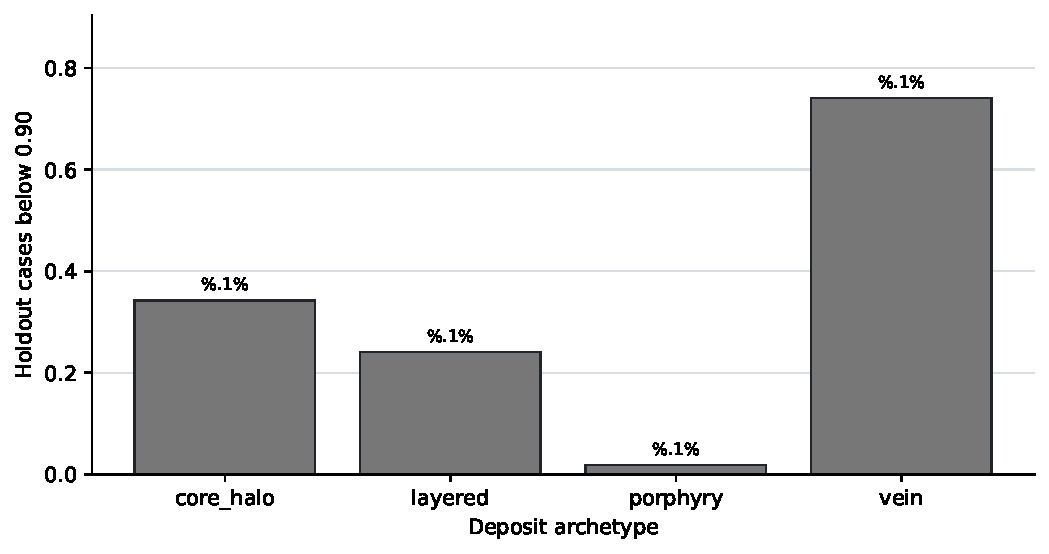
\includegraphics[width=0.82\textwidth]{figures/learned-failure-rate.pdf}\caption{Share of held-out generated cases below the fixed 0.90 value-ratio diagnostic, recomputed separately for each deposit archetype.}\label{fig:learned-failure-rate}\end{figure}
\clearpage

Figure~\ref{fig:learned-real-holdout} and Table~\ref{tab:real-holdout} retain the two benchmark cases separately: Newman1 is close to its exact expected-time comparator, while KD is below it. Two observations cannot estimate a cross-deposit transfer rate. The warning rule is also evaluated on a third disjoint set of 432 generated cases. Figure~\ref{fig:guard-confusion-matrix} shows 76 false negatives; Figure~\ref{fig:guard-thresholds} compares precision and recall with the frozen requirements, and Table~\ref{tab:guard-validation} includes the worst unflagged ratio. All three acceptance criteria fail. The warning rule therefore remains unavailable in the live lane; neither the figure nor the table supplies evidence for using it to screen real deposits.

\begin{figure}[htbp]\centering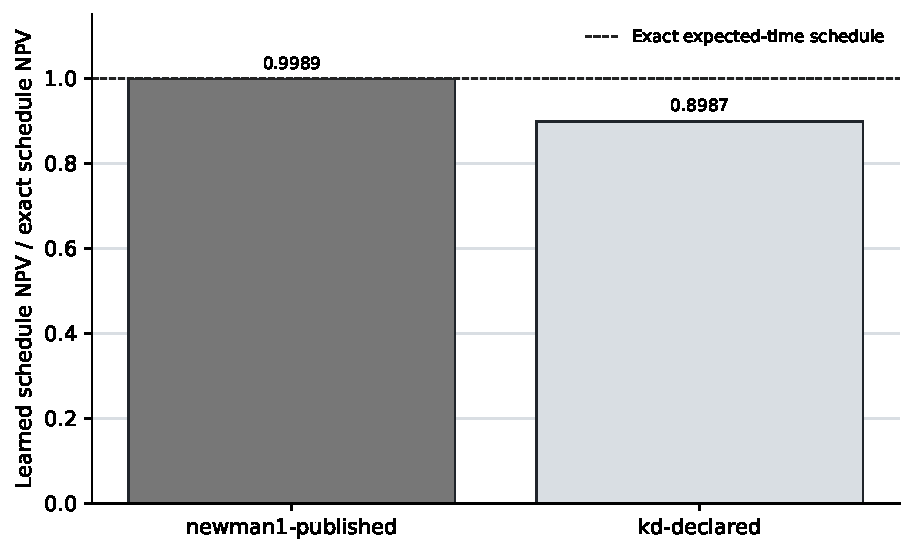
\includegraphics[width=0.7\textwidth]{figures/learned-real-holdout.pdf}\caption{Learned schedule value relative to exact expected-time ordering for the two scored MineLib cases, shown separately without pooling them into a transfer estimate.}\label{fig:learned-real-holdout}\end{figure}
\begin{figure}[htbp]\centering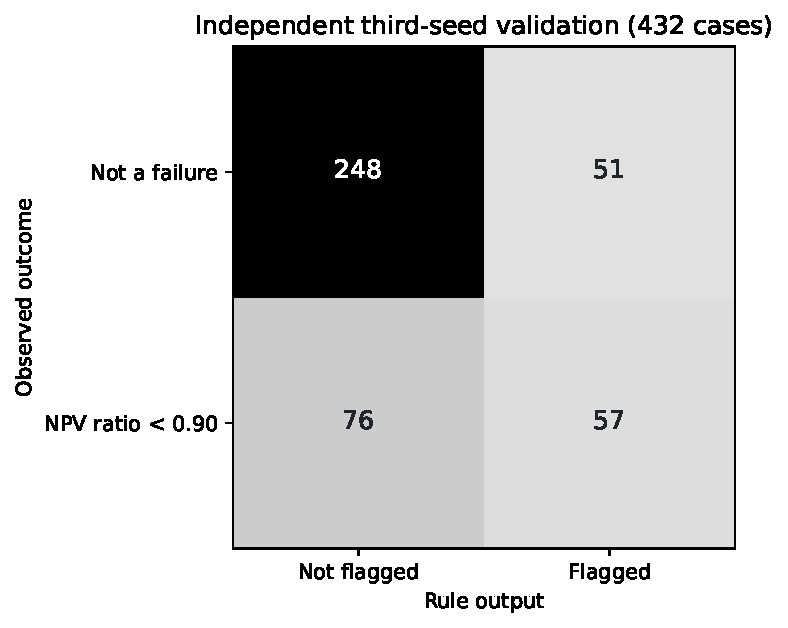
\includegraphics[width=0.66\textwidth]{figures/guard-confusion-matrix.pdf}\caption{Confusion matrix for the fixed archetype warning on its independent third-seed evaluation set, with missed low-value schedules visible explicitly.}\label{fig:guard-confusion-matrix}\end{figure}
\begin{figure}[htbp]\centering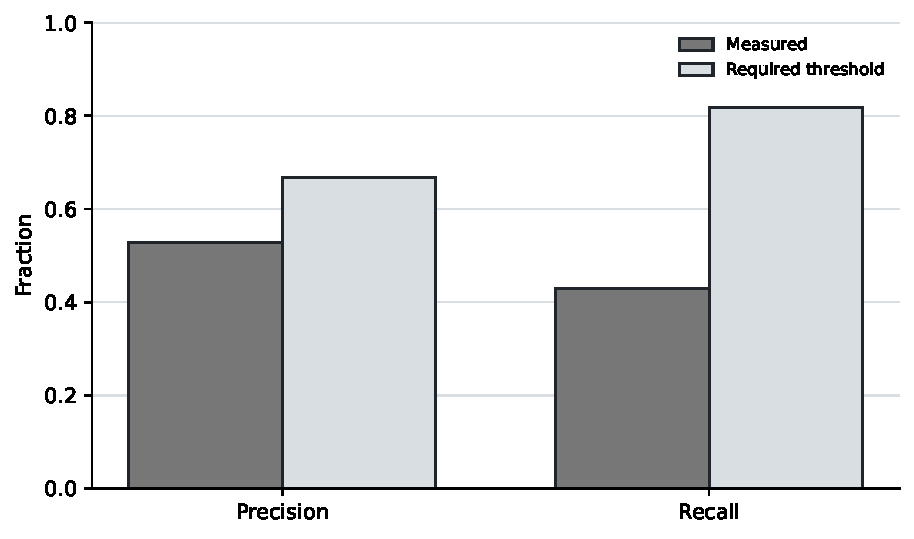
\includegraphics[width=0.72\textwidth]{figures/guard-thresholds.pdf}\caption{Measured guard precision and recall compared with the fixed acceptance thresholds defined before evaluation of the independent seed split.}\label{fig:guard-thresholds}\end{figure}

\begin{longtable}{lrrrrrr}
\caption{Deposit-disjoint synthetic evaluation results for the learned ordering and its exact comparator, grouped by archetype and measured on the same generated cases.}\label{tab:learned-by-archetype}\\
\toprule Archetype & $n$ & Median ratio & Mean ratio & 10th percentile & Minimum & Below 0.90 \\ \midrule
\endfirsthead\toprule Archetype & $n$ & Median ratio & Mean ratio & 10th percentile & Minimum & Below 0.90 \\ \midrule\endhead
core\_halo & 108 & 0.9348 & 0.9468 & 0.8482 & 0.7365 & 37/108 \\
layered & 108 & 0.9425 & 0.9337 & 0.8770 & 0.8536 & 26/108 \\
porphyry & 108 & 0.9972 & 1.0198 & 0.9484 & 0.8798 & 2/108 \\
vein & 108 & 0.8669 & 0.8600 & 0.7734 & 0.7101 & 80/108 \\
\bottomrule\end{longtable}

\begin{table}[htbp]\centering
\caption{The two licensed benchmark cases remain separate observations because they do not support an estimate of cross-deposit generalization.}\label{tab:real-holdout}
\begin{tabular}{lrrr}\toprule Case & Learned / exact ExTS & Spearman in pit & Scored \\ \midrule
newman1-published & 0.9989 & 0.2510 & yes \\
kd-declared & 0.8987 & 0.4214 & yes \\
\bottomrule\end{tabular}\end{table}

\begin{table}[htbp]\centering
\caption{The independently held-out warning rule is measured on 432 generated cases; the table preserves its false negatives and the thresholds it fails.}\label{tab:guard-validation}
\begin{tabular}{lrr}\toprule Measure & Measured & Required \\ \midrule
Precision & 0.5278 & $\geq 0.667$ \\
Recall & 0.4286 & $\geq 0.818$ \\
Worst unflagged ratio & 0.7322 & $\geq 0.7852$ \\
False negatives & 76 & 0 for complete detection \\
False positives & 51 & reported, not silently discounted \\
\bottomrule\end{tabular}\end{table}


\subsection{Reproducible system flow}
Figure~\ref{fig:system-architecture} maps the executable boundaries from case inputs through solving, independent evaluation, and the serialized replay products. The learned models are produced offline, while the deployed browser consumes static traces and uses its separate bounded interactive solver; the figure does not imply that the browser loads or trains the learned checkpoint. The source modules and contract schemas, rather than the diagram alone, define the exact data flow.

The first boundary is case admission: source dimensions, values, precedence, and capacities are converted into a versioned case description. The second boundary is method execution, which writes candidate schedules and solver outcomes without changing the source instance. The independent evaluator then recomputes feasibility and objective, and the contract layer serializes only the fields required for comparison and replay. The static site consumes the committed index and traces; it does not trigger a hidden full bake or update a published case when a reader changes a control. Synthetic interactive controls use a separately bounded calculation path and are visibly distinct from aggregate-only licensed benchmark records. These paths let readers distinguish a reproduced measurement, an interactive illustration, and a trained model artifact.

\begin{figure}[htbp]\centering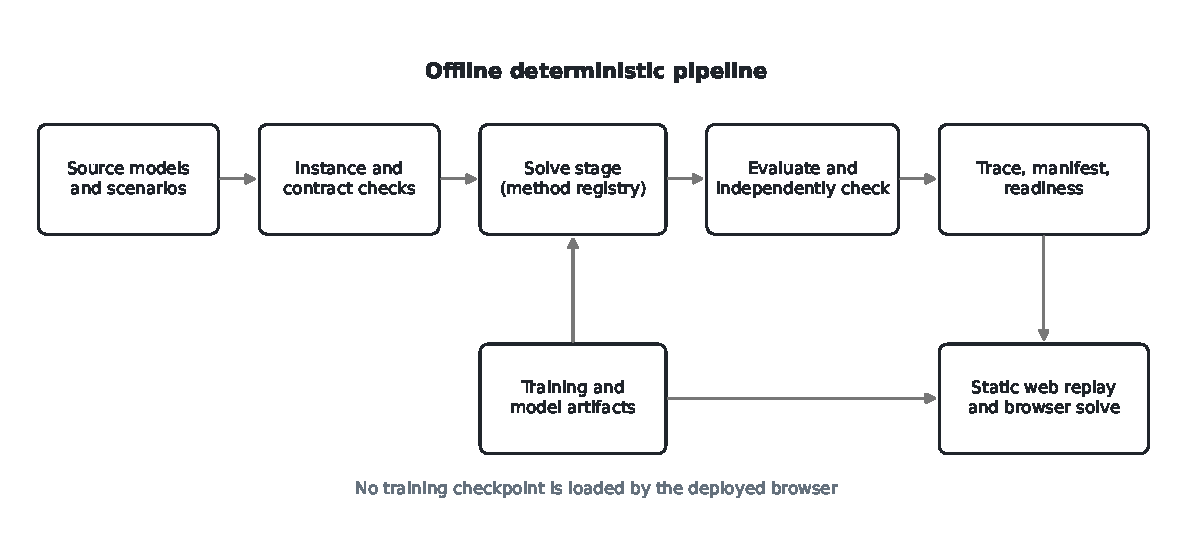
\includegraphics[width=\textwidth]{figures/system-architecture.pdf}\caption{PhaseFlow data path from model and scenario inputs through contract checks, registered solvers, independent evaluation, versioned traces, and browser replay.}\label{fig:system-architecture}\end{figure}

\section{Discussion}
The synthetic generator is not a geological simulator conditioned on drilling. The split supports transfer among its generated deposit families, not generalization to arbitrary mines. The classifier uses archetype information that may not be available for a real deposit. Small benchmark cases do not determine large-case computational cost. The expected-time prediction is not a bound, and its schedule is not a global optimum. The bound surrogate is visualization-only and cannot replace the exact bound at the selected point. Restricted neighborhood search and re-planning are heuristics. Re-planning uses one policy fixed before each draw and reports a lower bound on EVPI; it does not solve a two-stage stochastic program.
\section{Reproducibility and data availability}
Source code, automated validations, model files, derived traces, notebooks, and data contracts are maintained at \href{https://github.com/fsantibanezleal/CAOS_PhaseFlow}{CAOS PhaseFlow}. Python and TypeScript parity fixtures specify the supported computational paths. Synthetic data can be regenerated from the repository. MineLib block files are not redistributed; users must obtain them under source terms and configure an external data directory. Each trace records method versions, scenario, case identity, controls, and result values.
\section{Conclusions}
PhaseFlow places feasible construction heuristics, published scheduling methods, mathematical bounds, and a learned policy within one traceable benchmark. The learned policy produces useful schedules on many held-out generated cases, but its lower tail and vein failures preclude a general performance claim. Exact ExTS remains the nearest schedule comparator, and certified bounds remain the reference for optimality gaps. The policy is a fast candidate generator for cases where its assumptions hold; it does not replace mathematical certificates or mine-specific validation.
\begin{thebibliography}{9}
\bibitem{chicoisne} J. Chicoisne, D. Espinoza, M. Goycoolea, E. Moreno, and E. Rubio, ``A new algorithm for the open-pit mine production scheduling problem,'' \emph{Operations Research}, 60(3), 517--528, 2012. doi:10.1287/opre.1120.1050.
\bibitem{gershon} M. Gershon, ``Heuristic approaches for mine planning and production scheduling,'' \emph{International Journal of Mining and Geological Engineering}, 5, 1--13, 1987. doi:10.1007/BF01553529.
\bibitem{newman} W. B. Lambert, A. Brickey, A. M. Newman, and K. Eurek, ``Open-Pit Block-Sequencing Formulations: A Tutorial,'' \emph{Interfaces}, 44(2), 127--142, 2014. doi:10.1287/inte.2013.0731.
\bibitem{bienstock} D. Bienstock and M. Zuckerberg, ``Solving LP Relaxations of Large-Scale Precedence Constrained Problems,'' in \emph{Integer Programming and Combinatorial Optimization}, IPCO 2010, pp. 1--14. doi:10.1007/978-3-642-13036-6\_1.
\bibitem{blom} M. Blom, A. R. Pearce, and P. C\^ot\'e, ``Long-Term Open-Pit Mine Planning with Large Neighborhood Search,'' \emph{INFORMS Journal on Applied Analytics}, 56(2), 115--132, 2026. doi:10.1287/inte.2024.0152.
\bibitem{kingma} D. P. Kingma and J. Ba, ``Adam: A Method for Stochastic Optimization,'' arXiv:1412.6980, 2014.
\end{thebibliography}
\end{document}
